\documentclass[utf8]{beamer}
\usepackage{etex}
\usepackage{ctex}
%%%%%%%%%%%%%%%%%%%%%%%%%%%%%%%%%%%%%%%%%%%%%%%%%%%%%%%%%%%%%%%%%%%%%%%%%%
% There are a number of symbols (e.g., \Square) that are defined by      %
% multiple packages.  In order to typeset all the variants in this       %
% document, we have to give glyph a unique name.  To do that, we define  %
% \savesymbol{XXX}, which renames a symbol from \XXX to \origXXX, and    %
% \restoresymbols{yyy}{XXX}, which renames \origXXX back to \XXX and     %
% defines a new command, \yyyXXX, which corresponds to the most recently %
% loaded version of \XXX.                                                %
%                                                                        %

% Save a symbol that we know is going to get redefined.
\def\savesymbol#1{%
  \expandafter\let\expandafter\origsym\expandafter=\csname#1\endcsname
  \expandafter\let\csname orig#1\endcsname=\origsym
  \expandafter\let\csname#1\endcsname=\relax
}

% Restore a previously saved symbol, and rename the current one.
\def\restoresymbol#1#2{%
  \expandafter\let\expandafter\newsym\expandafter=\csname#2\endcsname
  \expandafter\global\expandafter\let\csname#1#2\endcsname=\newsym
  \expandafter\let\expandafter\origsym\expandafter=\csname orig#2\endcsname
  \expandafter\global\expandafter\let\csname#2\endcsname=\origsym
}

% Rather than create a rat's nest of \if statements, we keep the table
% whole and have each symbol conditionally appear.
\makeatletter
\newcommand{\trysym}[1]{\@ifundefined{#1}{\mbox{\tiny N/A}}{\csname#1\endcsname}}
\makeatother
%                                                                        %
%%%%%%%%%%%%%%%%%%%%%%%%%%%%%%%%%%%%%%%%%%%%%%%%%%%%%%%%%%%%%%%%%%%%%%%%%%

%---- usepackages ----
\usepackage{amscd}
\usepackage{amsmath,amssymb,amsfonts}%,mathrsfs}

% \usepackage{CJKutf8}
% \usepackage{CJKpunct,CJKspace}
% \punctstyle{CCT}
\usepackage{xcolor}
\usepackage{pgf,tikz}
\usepackage{graphicx}
\usepackage{subfigure}
%\usepackage{picins}  % 图片嵌入段落宏包 比如照片
%\usepackage{pstool} % for matlabfrag.m figures
\usepackage[english]{babel}
\usepackage[utf8]{inputenc}
\usepackage{times}
\usepackage[T1]{fontenc}
%\usepackage{booktabs}
% Or whatever. Note that the encoding and the font should match. If T1
% does not look nice, try deleting the line with the fontenc.
\usepackage{hyperref}
	\hypersetup{
		CJKbookmarks=true
		pdfpagemode={FullScreen}
	}
  \hypersetup{urlcolor=blue}
%---- set beamer page size to fit 16:9 or 16:10 screen ----
%---- uncomment next line for 16:9 aspect ratio ---
%\usepackage[orientation=landscape,size=custom,width=17.067,height=9.6,scale=0.5,debug]{beamerposter}
%---- uncomment next line for 16:10 aspect ratio ---
%\usepackage[orientation=landscape,size=custom,width=15.36,height=9.6,scale=0.5,debug]{beamerposter}

%---- 重定义字体、字号命令 ----
	% \newcommand{\songti}{\CJKfamily{song}}     % 宋体   (Windows自带simsun.ttf)
	% \newcommand{\kaishu}{\CJKfamily{kai}}      % 楷体   (Windows自带simkai.ttf)
	% \newcommand{\lishu}{\CJKfamily{li}}
	% \newcommand{\bodmtblk}{\CJKfamily{bodonimtblk}}
	% ---- 字号设置 ----
	\newcommand{\chuhao}{\fontsize{42pt}{\baselineskip}\selectfont}
	\newcommand{\xiaochuhao}{\fontsize{36pt}{\baselineskip}\selectfont}
	\newcommand{\yichu}{\fontsize{32pt}{\baselineskip}\selectfont}
	\newcommand{\yihao}{\fontsize{28pt}{\baselineskip}\selectfont}
	\newcommand{\erhao}{\fontsize{21pt}{\baselineskip}\selectfont}
	\newcommand{\xiaoerhao}{\fontsize{18pt}{\baselineskip}\selectfont}
	\newcommand{\sanhao}{\fontsize{15.75pt}{\baselineskip}\selectfont}
	\newcommand{\sihao}{\fontsize{14pt}{\baselineskip}\selectfont}
	\newcommand{\xiaosihao}{\fontsize{12pt}{\baselineskip}\selectfont}
	\newcommand{\wuhao}{\fontsize{10.5pt}{\baselineskip}\selectfont}
	\newcommand{\xiaowuhao}{\fontsize{9pt}{\baselineskip}\selectfont}
	\newcommand{\liuhao}{\fontsize{7.875pt}{\baselineskip}\selectfont}
	\newcommand{\qihao}{\fontsize{5.25pt}{\baselineskip}\selectfont}

\mode<presentation>
{
	%\usetheme{Warsaw}
	\usecolortheme{whale} % beaver, crane, wolverine - warm color theme
						% dove - black and white color theme
						% seahorse, shark - nice color theme
						% whale, dolphin - blue color theme, use 'outercolortheme' option for 'chamfered' inner theme
						% thu, EmoryBlue
	\usefonttheme{serif} % serif, structurebold, structuresmallcapsserif, professionalfonts
	\useinnertheme[realshadow]{chamfered}
	%\useinnertheme[realshadow, outercolortheme]{chamfered}
	\useoutertheme[nofootline]{wuerzburg}
	%\useoutertheme[nofootline, shadeframetitlebg]{wuerzburg}% options: glossy, nofootline, shadeframetitlebg
	\setbeamercovered{dynamic}
}

%---- setbeamertemplate ----
	%\setbeamertemplate[infolines theme]{headline}{}
	%\setbeamertemplate{footline}{} % ---- 删除底部信息条 ----
	% --删除底部导航工具栏, 替换为页数 或 logo--
	\usenavigationsymbolstemplate{\vbox{\hfill\structure{
		%\usebeamercolor[bg]{palette secondary}{\normalsize\bodmtblk\bfseries SUNIST}
		
\includegraphics[height=0.5cm]{logo/seu-color-logo.png}
		%\includegraphics[height=0.3cm]{logo/sunist-wolverine.pdf}
		%\includegraphics[height=0.3cm]{logo/sunist-thu.pdf}
		%\includegraphics[height=0.3cm]{logo/sunist-whale.pdf}
		%\tiny\insertframenumber{} / \inserttotalframenumber
	}\hspace{1ex}\vspace*{1ex}}}
%---- 设置背景渐变色 ----
%	\setbeamertemplate{background canvas}[vertical shading][bottom=structure.fg!15,top=white]
	%\setbeamertemplate{frametitle}[horizontal shading][left=blue, right=black]
%---- pictures dir ----
\graphicspath{{pics/}}

%---- sunist logo ----
	% \pgfdeclareimage[height=0.5cm]{thu}{thu.JPG}
	% \logo{\pgfuseimage{thu}}
	%or
	%\logo{\includegraphics[height=0.3cm]{sunistlogo2.pdf}}

% Delete this, if you do not want the table of contents to pop up at
% the beginning of each subsection:
\AtBeginSubsection[]
{
	\begin{frame}<beamer>
		\frametitle{Outline}
		\tableofcontents[currentsection,currentsubsection]
	\end{frame}
}

% If you wish to uncover everything in a step-wise fashion, uncomment
% the following command:
%\beamerdefaultoverlayspecification{<+->}

%---- includeonlyframes ----
%\includeonlyframes{inclonlyframelabel}

%---- set paragraph skip ----%
\setlength{\parskip}{1ex  plus  0.5ex  minus  0.2ex}

% ---- Change the bullets ----
\useitemizeitemtemplate{%
    \tiny\raise1.5pt\hbox{{$\blacksquare$}}%
}
\usesubitemizeitemtemplate{%
    \tiny\raise1.5pt\hbox{{$\blacklozenge$}}%
}
\usesubsubitemizeitemtemplate{%
    \tiny\raise1.5pt\hbox{{$\blacktriangleright$}}%
}
%\usesubsubsubitemizeitemtemplate{%
%    \tiny\raise1.5pt\hbox{{$\bullet$}}%
%}
% Plot a tiny plasma current graph
% Input:
%   #1 Plot data
%   #2 Mean current
\newcommand{\dataplot}[2]{%
    \begin{tikzpicture}[xscale=0.5, yscale=0.03]
        \begin{scope}[ycomb, yscale=0.5]
        	\draw[densely dotted, thin, black!50] (35,0)--(40,0);
            \draw[densely dotted, thin, black!50] (35,#2)--(40,#2);
            \draw[ultra thin, black!80] plot[smooth] #1;
            \node[above left, scale=0.35] at (35,0) {$0$};
            \node[below left, scale=0.35] at (35,#2) {$#2$};
        \end{scope}
    \end{tikzpicture}%
}

%\pgfdeclarehorizontalshading[frametitle.bg]{beamer@frametitleshade}{1em}{%
%	color(0pt)=(frametitle.bg);
%	color(\paperwidth)=(white)
%}

\newcommand{\thankyoupage}[1]{%
	\begin{frame}
		\begin{centering}
		\begin{beamercolorbox}[sep=3pt,center]{title}
			\usebeamerfont{title}\inserttitle\par%
			\ifx\insertsubtitle\@empty%
			\else%
				\vskip0.25em%
				{\usebeamerfont{subtitle}\usebeamercolor[fg]{subtitle}\insertsubtitle\par}%
			\fi%
		\end{beamercolorbox}%
		\end{centering}
		\vskip2em\par
		\begin{centering}
		\hfill
		\begin{beamercolorbox}[wd=0.8\linewidth,center,rounded=true]{palette secondary}
			\usebeamerfont{title  in  head/foot}
			\huge{#1}
		\end{beamercolorbox}
		\hfill
		\end{centering}
	\end{frame}
}

\newcommand<>{\hover}[3]{\uncover#4{%
	\begin{tikzpicture}[remember picture,overlay]%
		\draw[fill,opacity=0.4] (current page.south west)
			rectangle (current page.north east);
		\node at (current page.center) {%
			\begin{minipage}{{#1}}
			\begin{block}{{#2}}
				{#3}
			\end{block}
			\end{minipage}
		};
	\end{tikzpicture}}
}

\newcommand{\myfootnote}[1]{\footnote{\tiny{{#1}}}}

\newcommand{\backupframebegin}{
     \newcounter{framenumberbeforeappendix}
     \setcounter{framenumberbeforeappendix}{\value{framenumber}}
     \setbeamertemplate{headline}[wuerzburg theme appendix]
     \setbeamertemplate{footline}[wuerzburg theme appendix]
}
\newcommand{\backupframeend}{
   \addtocounter{framenumberbeforeappendix}{-\value{framenumber}}
   \addtocounter{framenumber}{\value{framenumberbeforeappendix}}
   \setbeamertemplate{headline}[wuerzburg theme]
   \setbeamertemplate{footline}[wuerzburg theme]
}


\usepackage{booktabs}%, makecell}
\usepackage{overpic}
\usepackage{multirow}
\usepackage{makecell}
%\usepackage{colortbl}
%\usepackage{transparent}
%\usepackage{fixpauseincludegraphics}
\usepackage{siunitx}
\usepackage{tabu}
\usepackage{caption}
\captionsetup{font=scriptsize,labelfont=scriptsize}
\usepackage{bm}


\setbeamertemplate{background canvas}[vertical shading][bottom=white,top=white]
\setbeamertemplate{caption}{\raggedright\insertcaption\par}

\AtBeginSection[]
{
  \begin{frame}<beamer>
    \frametitle{提纲}
    \tableofcontents[sections={2-},currentsection,subsectionstyle=show/show/hide]%,sections={2-6}]
  \end{frame}
  \addtocounter{framenumber}{-1}
}

\AtBeginSubsection[]
{
  \begin{frame}<beamer>
    \frametitle{提纲}
    \tableofcontents[sections={2-},currentsection,subsectionstyle=show/shaded/hide]
  \end{frame}
  \addtocounter{framenumber}{-1}
}

\newcommand{\onlineref}[1]{{\scriptsize\texttt{[#1]}}}

%\setbeamerfont{itemize/enumerate body}{font=\bf}

%---- 自定义或重定义环境等,一般用于中文幻灯片 ---
% \newenvironment{dingyi}{definition} %自定义环境
\newcommand{dingyi}[definition]{定义}
\newtheorem{li}{例}
\newenvironment{Definition}{\begin{definition}}{\end{definition}}
\def\theoremname{定理}
\def\defname{定义}
\def\lemmaname{引理}
\def\proofname{证明}
\def\corollaryname{推论}
\def\examplename{例}
\newtheorem{proposition}{命题}
\renewcommand\figurename{\rm 图}
\renewcommand\tablename{\bf 表}





\begin{document}
% \begin{CJK*}{UTF8}{kai}

\title[硕士学位论文答辩]{大跨越输电塔结构在龙卷风作用下的响应分析}

% \author{140926~王勇 \\[1.5 \baselineskip]  \footnotesize{导师: 吕令毅 ~ 教授}}

\author[王勇]{
  \quad
  \begin{minipage}{4cm}
    硕士生:王 勇\\
    导\quad 师:吕令毅\quad 教授
  \end{minipage}
}

\institute{东南大学土木工程学院}

\date{2017-06-01}

\frame{\titlepage}

\section*{提纲}
\frame{\frametitle{提纲}\tableofcontents[sections={2-},hideallsubsections]}

%%%%%%%%%%%%%%%%%%%%%%%%%%%%%%%%%%%%%%%%%%%%%%%%%%%%%%%%%%%%%%%%%%%%%%%%%%%%%

\section{引言}
\subsection{课题研究背景与意义}

\begin{frame}
  \frametitle{2016年江苏盐城龙卷风灾害}
  \begin{figure}
    \centering
    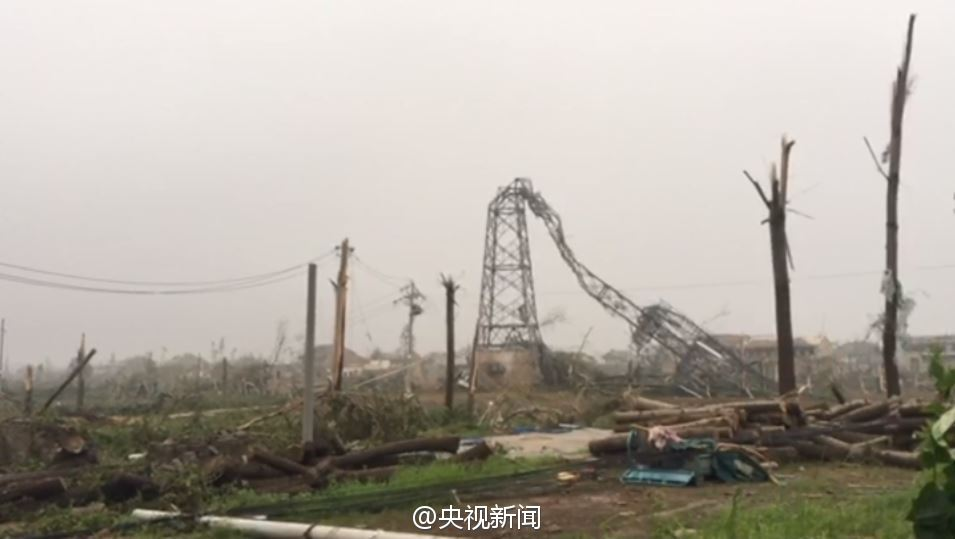
\includegraphics[width=\textwidth]{yancheng2.jpg}
    \caption*{2016年江苏盐城龙卷风中输电塔破坏\\ \url{http://society.people.com.cn/n1/2016/0623/c1008-28473500.html}}
    
  \end{figure}
\end{frame}

\begin{frame}
  \frametitle{2016年江苏盐城龙卷风灾害}
  \begin{itemize}
  \item
    共计 220 座各类通信基站退服,倒杆 2800 根,
    部分地区出现影响电力供应中断和通信基站无信号的情况,1570 根有线信号杆线受损,
    162 杆路灯损坏,40 条高压供电线路受损,影响 3 万负荷供电。
  \item
    射阳县电力、通讯杆线受损严重,龙卷风经过的 4 条 10 千伏线路区域用户全停。\\
    {\scriptsize \url{http://www.thepaper.cn/newsDetail_forward_1488127}}
  \bigskip
  \item
    输电线路的破坏直接影响了救援救伤的效率,造成了灾区人民生命财产的重大损失。
  \end{itemize}
  
\end{frame}

\begin{frame}
  \frametitle{课题研究背景与意义}
  \begin{itemize}
  \item
    大跨越输电塔结构是重要的生命线电力工程设施 ,具有数量大、分布广等特点,容易遭受龙卷风的袭击。
  \item
    全球范围内约 $80\%$ 的输电塔倒塌破坏是由于极端天气(如龙卷风、雷暴等)的影响。
  \item
    输电塔结构破坏将导致供电系统的瘫痪甚至引发火灾等严重后果,造成重大经济损失。
  \bigskip
  \item
  鉴于近年龙卷风发生频率和强度似有增大趋势,而以往国内针对输电塔受龙卷风袭击的研究较少,故为保障龙卷风多发地区电网运行安全,进行输电线路的龙卷风荷载及抗风研究具有重要的理论和实用价值。

  \end{itemize}
 
\end{frame}

\subsection{课题研究思路与内容}
\begin{frame}
  \frametitle{课题研究思路与内容}
  \begin{figure}
    \centering
    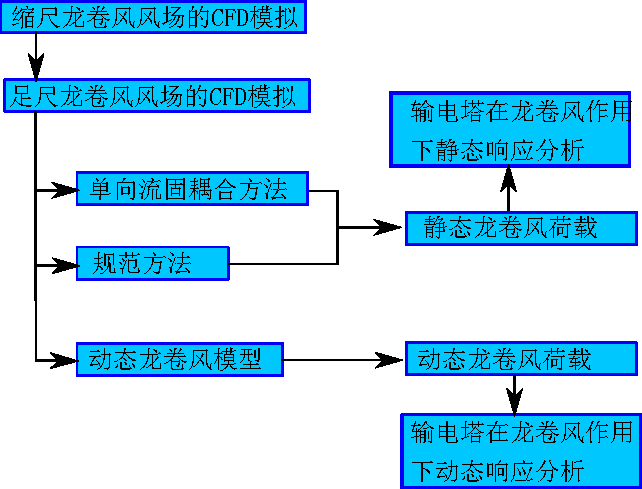
\includegraphics[height=0.8\textheight]{flow_chart.pdf} 
  \end{figure}
\end{frame}

\section{龙卷风风场及其数值模拟}
\subsection{缩尺龙卷风的CFD模拟}

\begin{frame}
  \frametitle{风场几何区域}

  \begin{columns}
    \column{0.5\textwidth} 
    \begin{figure}
      \centering
      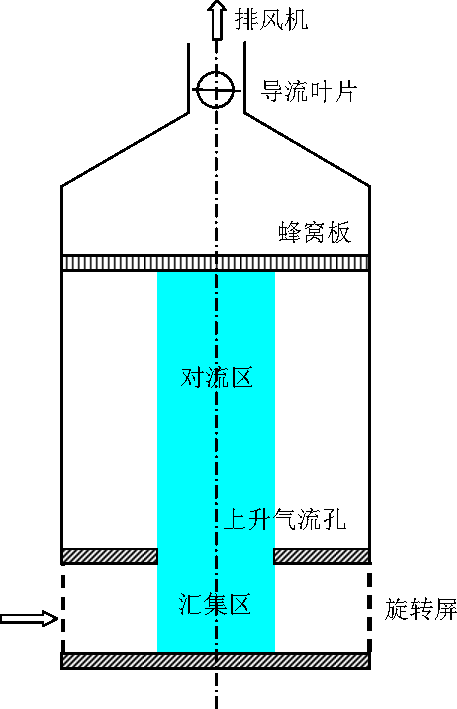
\includegraphics[height=0.5\textheight]{Ward_TVC_sketch.pdf}
      \caption*{Purdue龙卷风发生装置示意图}
      \label{fig:Ward-TVC}
    \end{figure}
   
    \column{0.5\textwidth} 
    \begin{figure}
      \centering
      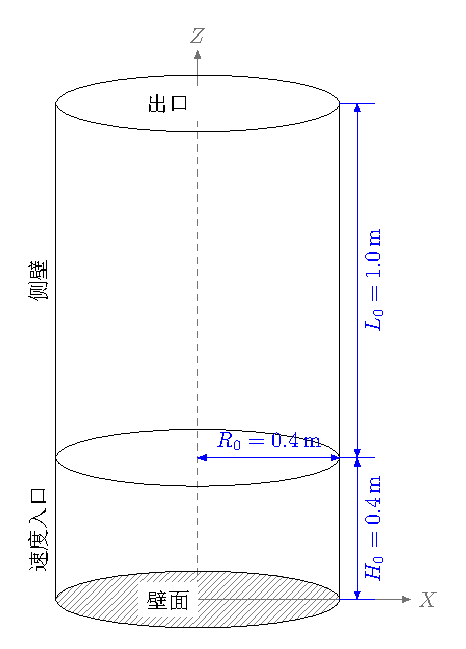
\includegraphics[height=0.5\textheight]{domain.pdf}
      \caption*{龙卷风CFD模拟计算流域}
      \label{fig:TVC-domain}
    \end{figure}
  \end{columns}

  \begin{columns}
    \column{0.45\textwidth}
    \begin{description}
    \item[高宽比] $A = H_0/R_0$ 
    \item[涡流比] $S = V_t/2A V_r$
    \end{description}

    \column{0.55\textwidth}
    \begin{description}
    \item[$V_t$] $R_0$ 处切向入流速度
    \item[$V_r$] $R_0$ 处径向入流速度
    \end{description}
  \end{columns}

\end{frame}

\begin{frame}
  \frametitle{CFD边界条件设置}

  速度入口处径向和切向速度分布采用如下形式:
  \begin{equation}\label{eqn:Vr}
    V_r(z) = V_0 \times (z/z_0)^{1/7}
  \end{equation}
  \begin{equation}\label{eqn:Vt}
    V_t(z) = 2 \times S \times V_r(z)
  \end{equation}
  式中,$V_0$为参考速度,$z_0$为参考高度,$S$为涡流比。

  \begin{figure}
    \centering
    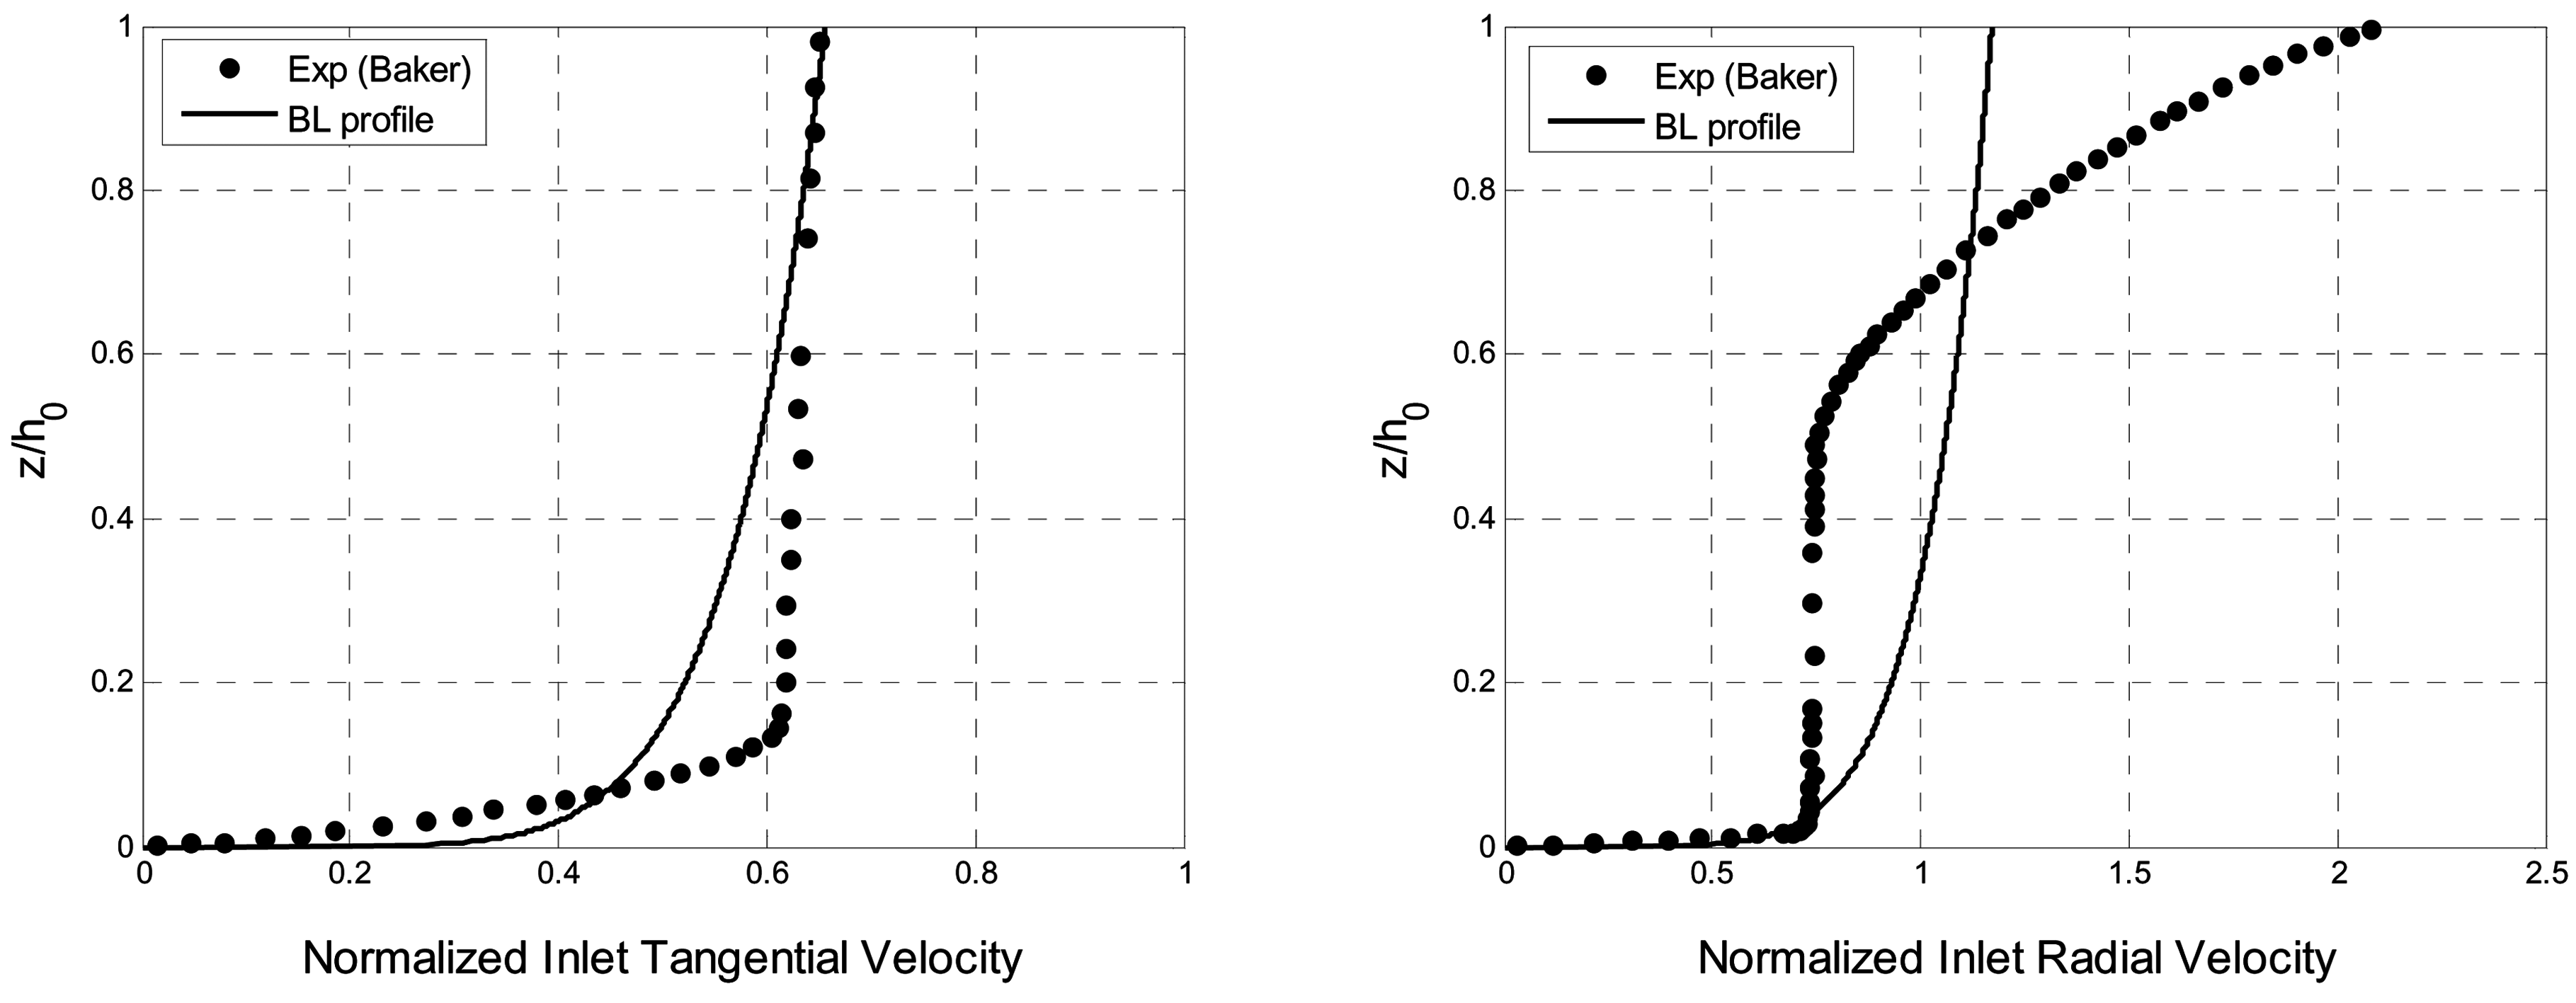
\includegraphics[height=0.5\textheight]{bc_inlet.png}
    \caption*{CFD速度入口规格化切向和径向速度与Baker试验的对比}
    \label{fig:bc-inlet}
  \end{figure}
\end{frame}

\subsection{缩尺龙卷风数值模拟结果及正确性验证}

\begin{frame}
  \frametitle{CFD模拟风场与Baker试验的对比} 
  Baker利用Purdue试验装置进行了龙卷风风场的试验模拟,选取$S=0.28$的风场在$r/R_0=0.1025$和$r/R_0=0.2125$处风速各分量随高度变化曲线与数值风场进行对比。
  \begin{figure}[!htbp]
    \centering
    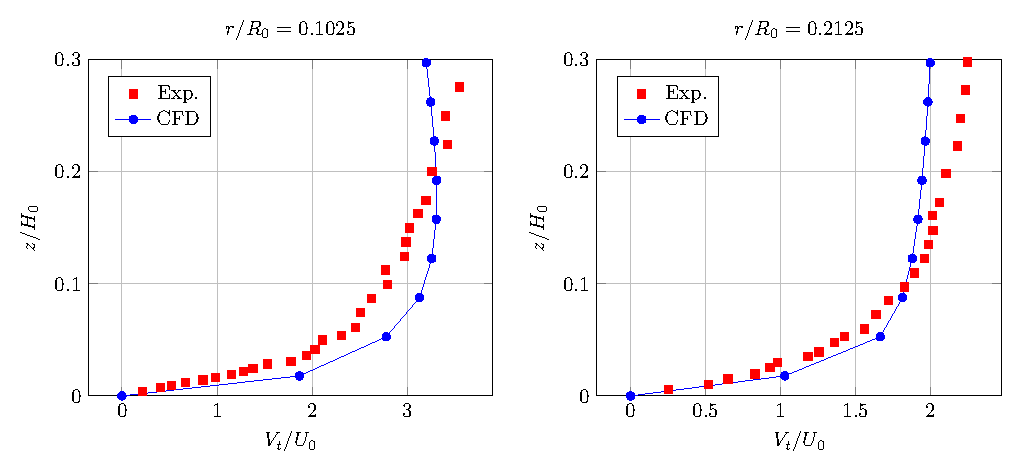
\includegraphics[height=0.5\textheight]{cfd_vs_exp_Vt.pdf}
    \caption*{数值风场与Baker试验无量纲化切向速度随高度变化的对比,$S=0.28$}
    \label{fig:cfd_vs_exp_Vt}
  \end{figure}
\end{frame}

\begin{frame}
  \frametitle{数值龙卷风的风速分布}
  \begin{figure}
    \centering
    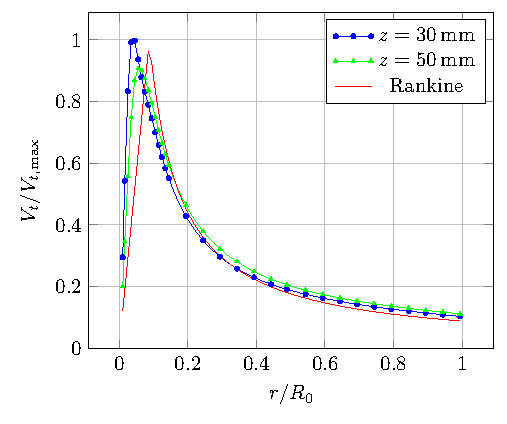
\includegraphics[height=0.7\textheight]{Vt.pdf}
    \caption*{数值风场不同高度处切向速度沿径向的变化图,$S=0.28$}
    \label{fig:Vt}
  \end{figure}

  % 由图\ref{fig:Vt}可知龙卷风涡旋中心的切向速度较小,在核心半径处达到最大,而后随着远离涡旋中心的距离增大而逐渐减小。
  % 且在核心半径内,切向速度的变化较快,而远离核心半径时,变化逐渐缓和,与Rankine模型吻合较好。
  % 此外还可看出随着离地高度的增加,核心半径有所增大,而最大切向风速呈逐渐减小的趋势。

\end{frame}

\begin{frame}
  \frametitle{数值龙卷风的风速分布}

  \begin{figure}[!htbp]
    \centering
    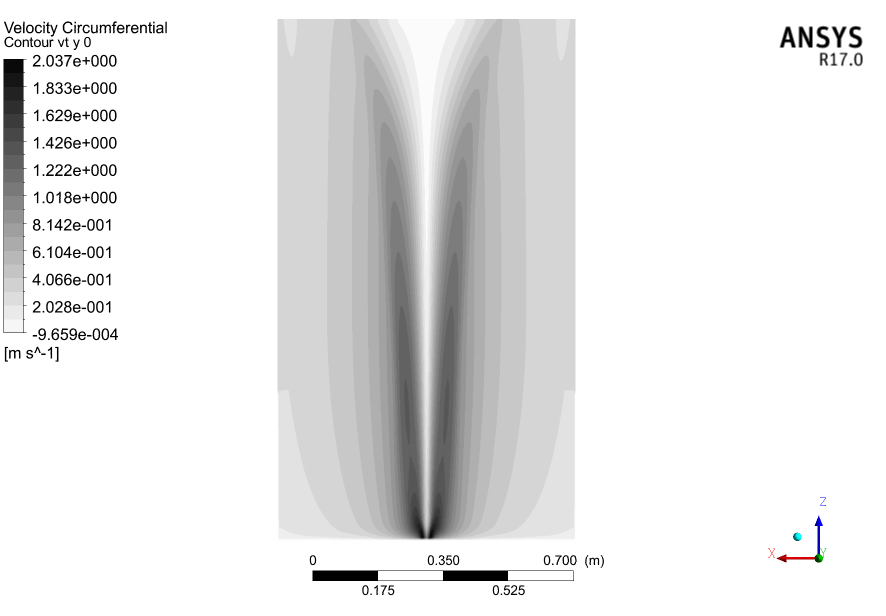
\includegraphics[height=0.7\textheight]{Vt_y=0.png}
    \caption*{轴向剖面($Y=0$)处切向风速云图}
    \label{fig:Vt-x=0}
  \end{figure}

  % 图\ref{fig:Vt-x=0}为计算流域轴向剖面($X=0$)处切向速度云图。
  % 从图中可以明显看出涡旋中心处切向速度接近于零。

\end{frame}

\subsection{足尺龙卷风的CFD模拟}

\begin{frame}
  \frametitle{长度相似比和速度相似比}
  \begin{itemize}
  \item
    足尺风场选用1998年5月发生在美国南达科他州Spencer地区的实测龙卷风风场。 
  \item
    考虑缩尺风场和实测风场的最大切向速度及其发生位置$V_t(r_{c\,\mathrm{max}}, z_{\mathrm{max}})$,
    其中$r_{c,\mathrm{max}}$为风场在$z_{\mathrm{max}}$高度处的核心半径。
  \item
    速度相似比和长度相似比定义为:
    \begin{equation}
      V_s  =  \frac{V_{t,\mathrm{max}}^{\text{Full}}}{V_{t,\mathrm{max}}^{\text{CFD}}}
    \end{equation}
    \begin{equation}
      L_s  =  \frac{r_{c,\mathrm{max}}^{\text{Full}}}{r_{c,\mathrm{max}}^{\text{CFD}}} \quad \text{or} \quad \frac{z_{c,\mathrm{max}}^{\text{Full}}}{z_{c,\mathrm{max}}^{\text{CFD}}}
    \end{equation}  
  \item
    本文模拟的缩尺龙卷风速度相似比为$V_s=60$,长度相似比为$L_s=4000$。
  \end{itemize}
  
\end{frame}

\begin{frame}
  \frametitle{足尺龙卷风风场CFD模拟}
  利用长度相似比$L_s$和速度相似比$V_s$将缩尺CFD风场转化为足尺龙卷风风场(
  缩尺风场的计算流域几何尺寸放大$L_s$倍;
  入口边界条件的径向和切向入流速度放大$V_s$倍)
  \begin{figure}[!htbp]
    \centering
    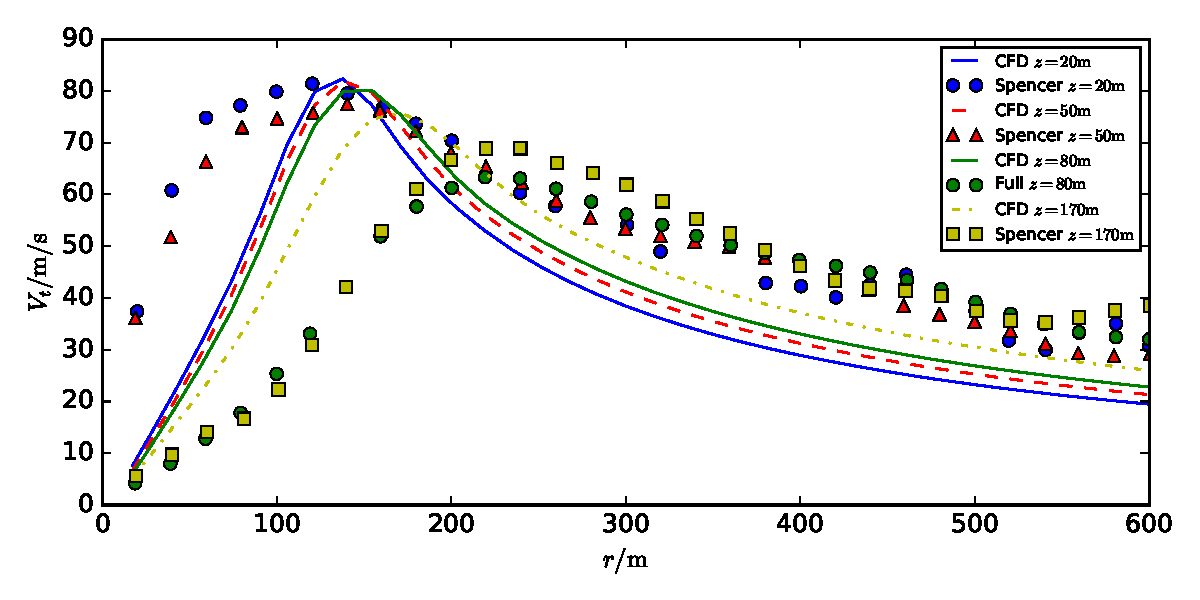
\includegraphics[height=0.6\textheight]{cfd-vs-Spencer.pdf}
    \caption*{CFD足尺风场与Spencer实测风场切向速度分布比较}
    \label{fig:cfd-Spencer}
  \end{figure}

\end{frame}

\section{输电塔结构在龙卷风作用下的静态响应分析}
\subsection{输电塔结构有限元建模}

\begin{frame}
  \frametitle{输电塔结构有限元建模}
  
  \begin{figure}[!htbp]
  	\centering
    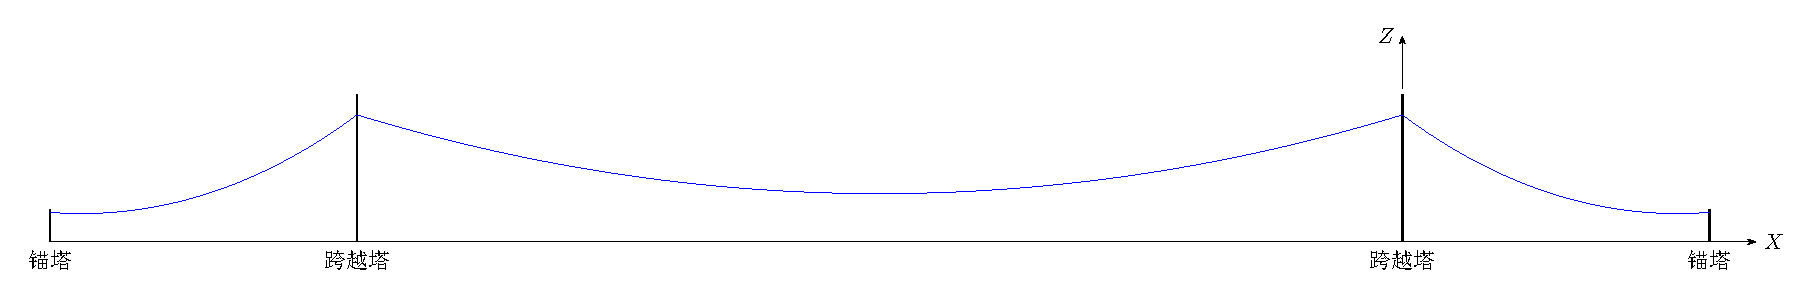
\includegraphics[width=\textwidth]{tower_line_system.pdf}
    % \caption{三江口大跨越示意图}
    \label{fig:tower-line}
  \end{figure}

  \begin{itemize}
  \item
    选择跨越塔为研究对象。南北跨越塔均为双回路蝶形布置的钢管塔,呼高\SI{215}{m},全高\SI{249.5}{m},根开\SI{49.6}{m}。
  \item 
    选用二节点非线性三维梁单元BEAM 188模拟输电塔构件。
    单元每个节点处包括三个平动自由度和三个转动自由度。
    输电塔构件之间为多孔螺栓连接,有限元模型以刚性节点模拟。
  \item
   考虑到输电塔为空间对称结构,取塔的底面中心为坐标原点,高度方向为$Z$轴方向,输电线方向为$X$轴方向。
  \end{itemize}

\end{frame}

\begin{frame}
  \frametitle{输电塔有限元模型模态分析}
  
  \begin{figure}[!htbp]
    \centering
    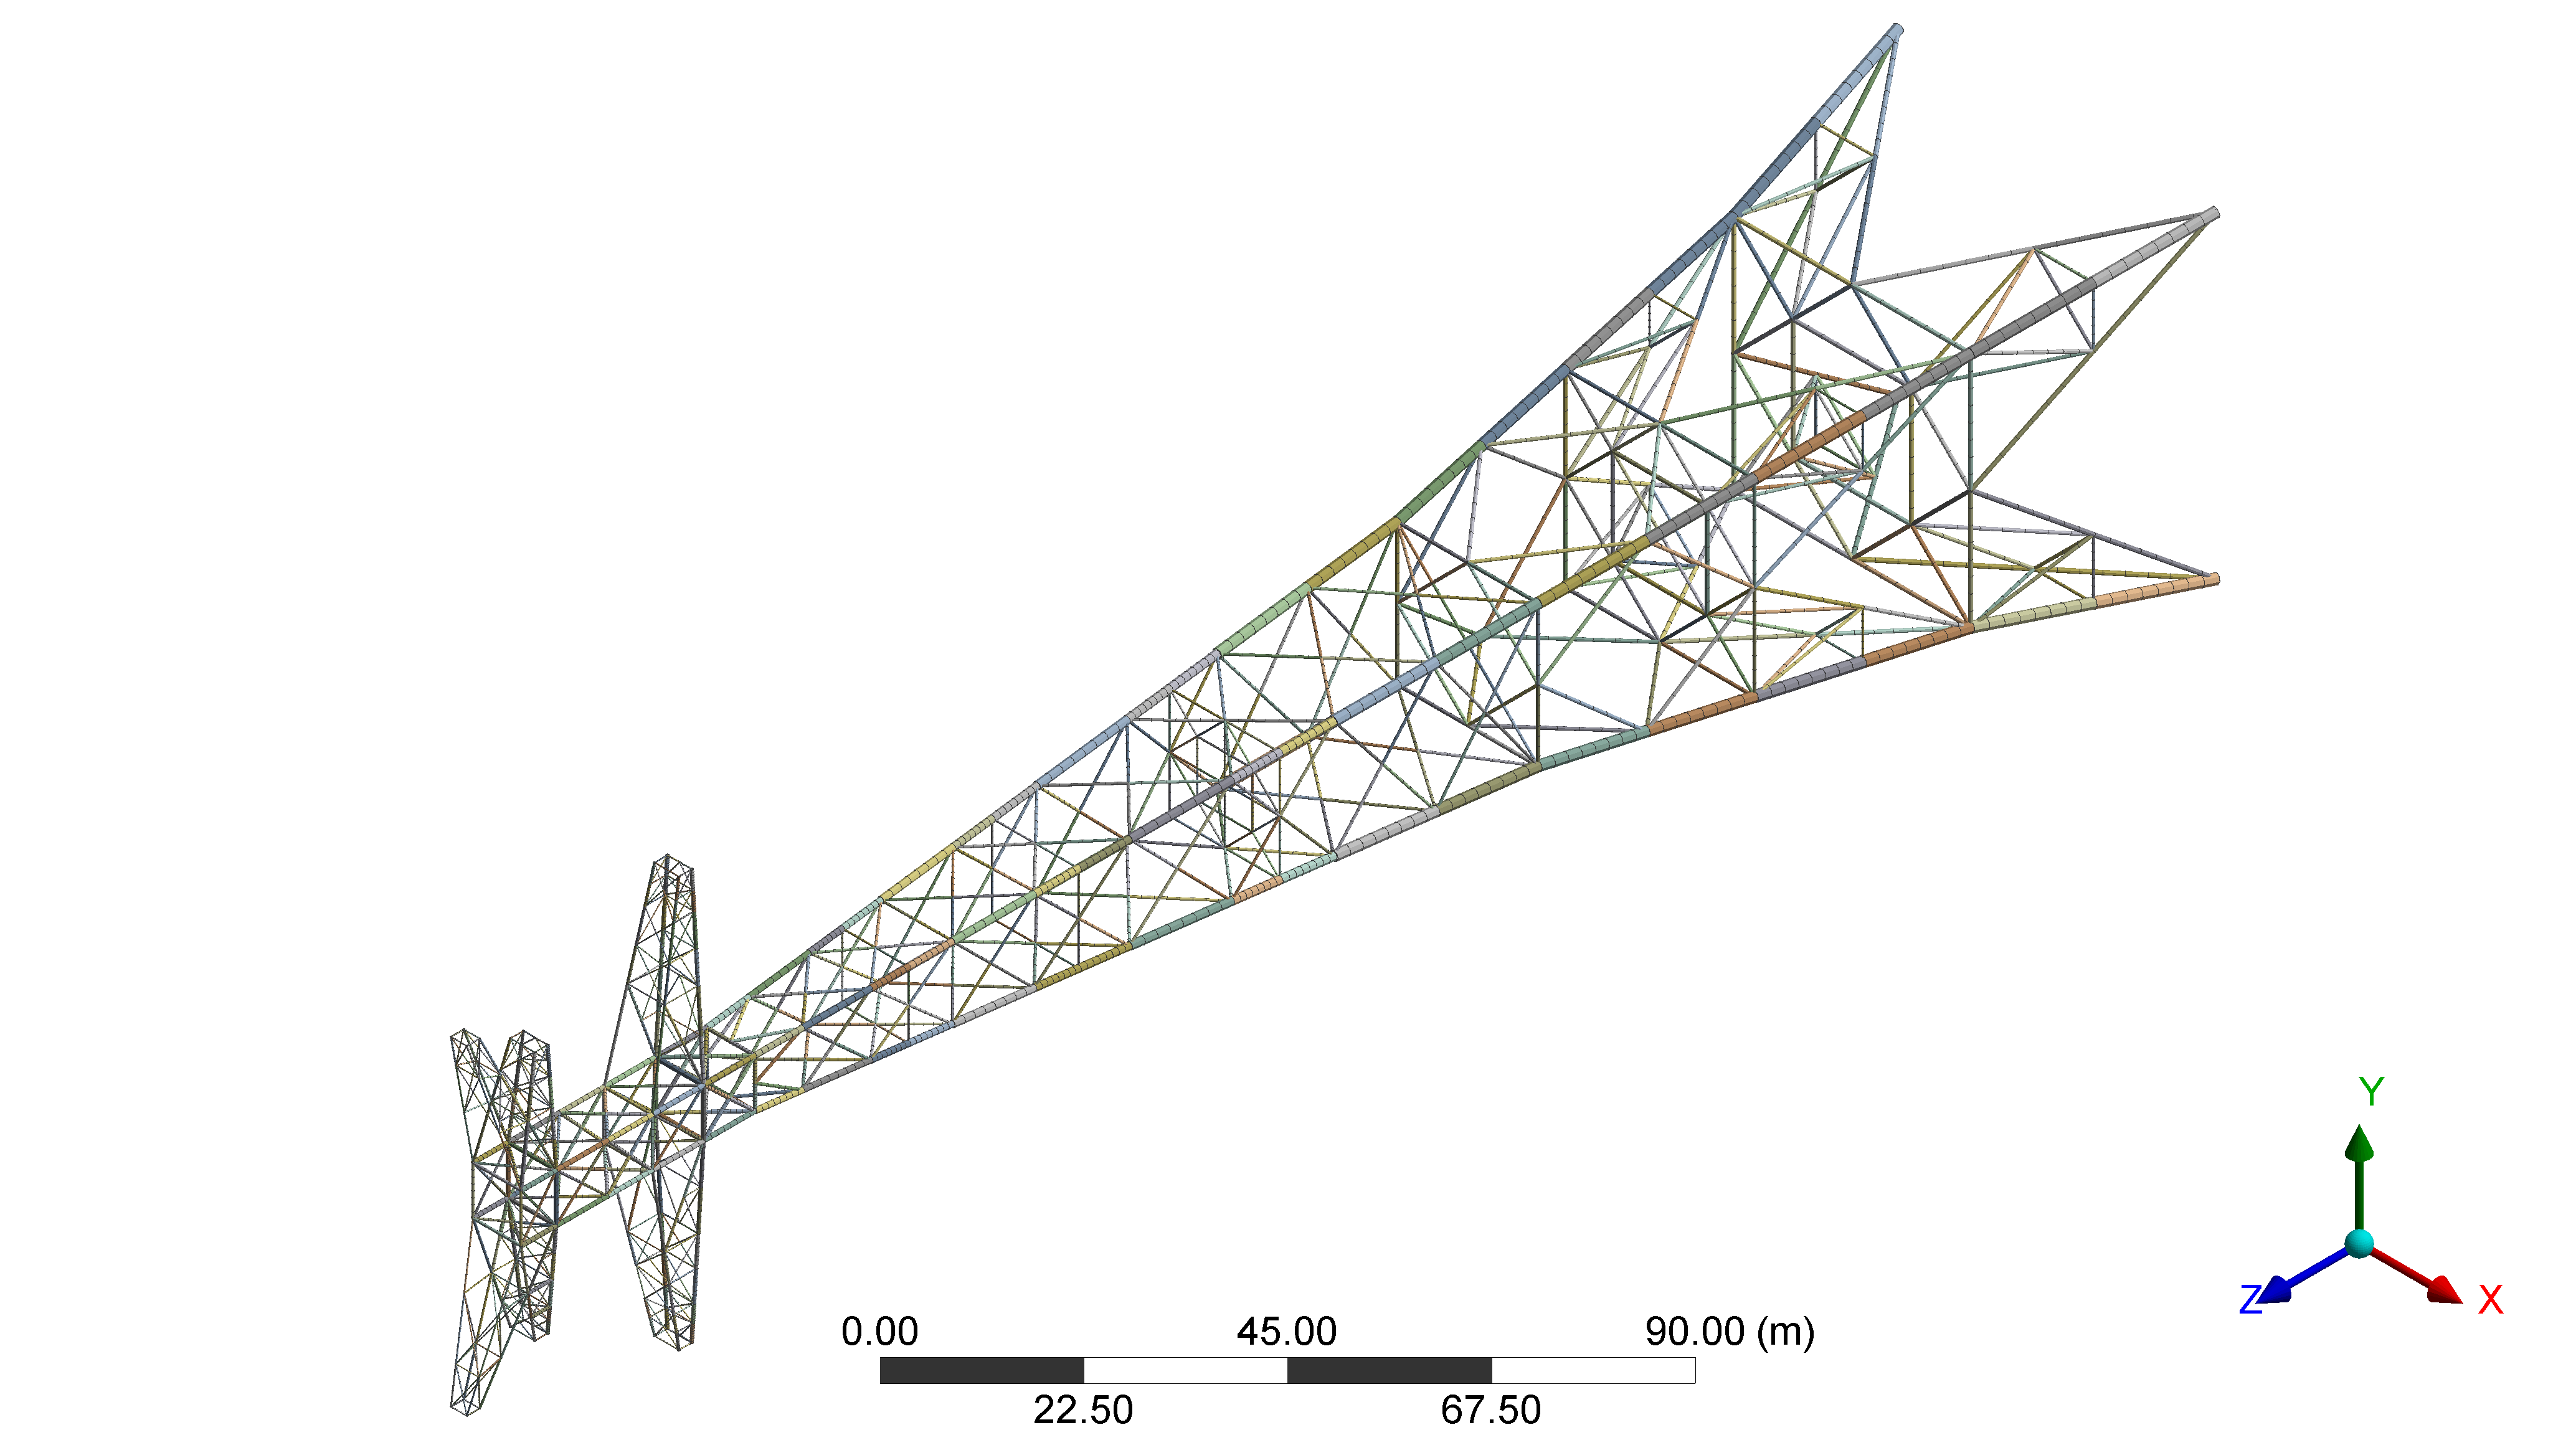
\includegraphics[height=0.5\textheight]{tower_fea.png}
    % \caption{输电塔有限元模型}
    \label{fig:tower-fea}
  \end{figure}

  \begin{table}[!htbp]
	\centering
	% \caption*{输电塔自振频率$(\SI{}{Hz})$}
	\label{tab:freq}
	\begin{tabu} to 1.0\textwidth {X[1.5,c] X[1,c] X[1,c] X[1,c] X[1,c] X[1,c] X[1,c] X[1,c] X[1,c] X[1,c]}
		\toprule
		振型 & 1     & 2     & 3     & 4     & 5     & 6     & 7     & 8     & 9     \\
		\midrule
		频率 & 0.609 & 0.612 & 1.102 & 1.558 & 1.608 & 2.113 & 2.296 & 2.407 & 3.046 \\
    文献 & 0.613 & 0.615 & 1.093 & 1.565 & 1.594 & 2.084 & 2.312 & 2.363 & 2.368 \\
		\bottomrule
	\end{tabu}
\end{table}

\end{frame}

\subsection{输电塔龙卷风荷载计算的FSI方法}

\begin{frame}
  \frametitle{输电塔龙卷风荷载计算的FSI方法}

  \begin{itemize}
  \item 
    单向流固耦合分析(One-way Fluid Structure Interaction, FSI)
    \begin{itemize}
    \item
      首先,将结构表面视为刚性的流场壁计算流场的分布;
    \item
      然后将流场计算得到的刚性壁面压力施加到结构上以计算其响应。
    \end{itemize}
    \bigskip
  \item
    输电塔结构分为主体框架和支撑体系
    \begin{itemize}
    \item
      输电塔主体框架迎风效应较大,直接在CFD风场中建立刚性模型,进行FSI计算;
    \item
      支撑等构件迎风效应较小,通过提取CFD风场速度利用风荷载公式计算。

    \bigskip
    \item
      可降低网格划分难度,减小CFD计算量。
    \end{itemize}
  \end{itemize}

\end{frame}

\begin{frame}
  \frametitle{包含输电塔刚性模型的龙卷风风场}
  \begin{figure}
    \centering
    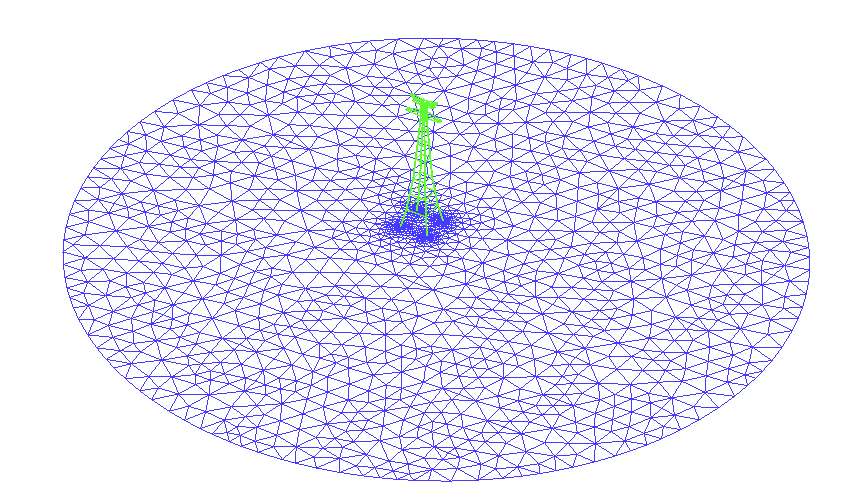
\includegraphics[height=0.5\textheight]{mesh.png}
    \caption*{输电塔周围计算流域网格}
  \end{figure}

  \begin{itemize}
  \item
    控制输电塔表面网格划分的最大单元尺寸为\SI{0.4}{m}。
  \item 
    输电塔表面设置厚度为1.0m的棱柱形单元膨胀层网格。
  \item
    以输电塔中心建立半径为\SI{150}{m}的球状区域,在此区域内进行网格加密以尽可能精确离散结构表面。
  \end{itemize}
\end{frame}

\begin{frame}
  \frametitle{输电塔主体框架受到的龙卷风风压}

  \begin{columnsonlytextwidth}
   \column{0.5\textwidth} 
      \begin{figure}[!htpb]
     \centering
     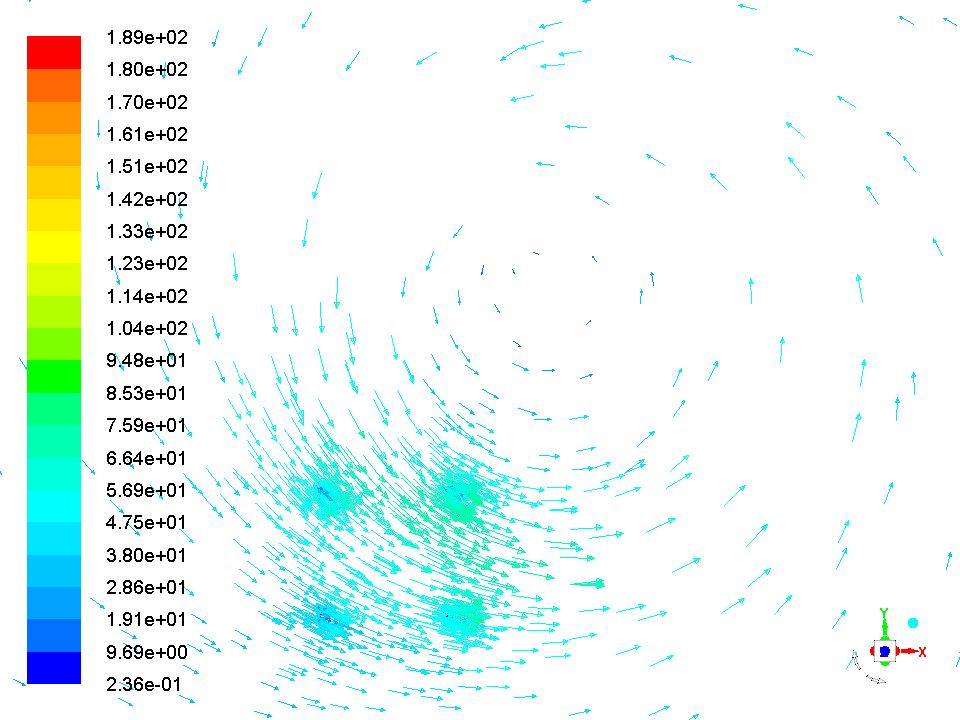
\includegraphics[height=0.5\textheight]{velo.jpg}
     \caption*{\SI{20}{m}高度处风速矢量图}
     \label{fig:velocity}
   \end{figure}

   \column{0.5\textwidth}
   \begin{figure}[!htpb]
     \centering
     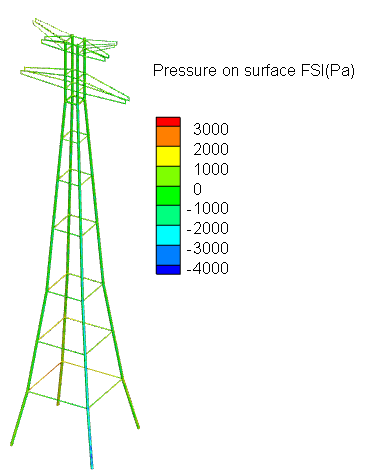
\includegraphics[height=0.8\textheight]{pres.png}
     \caption*{输电塔表面风压}
     \label{fig:pressure}
   \end{figure}

  \end{columnsonlytextwidth}
  
\end{frame}
\begin{frame}
  \frametitle{输电塔主体框架龙卷风风压转化为梁单元节点集中力}

  % \begin{figure}[!htbp]
  %   \centering
  %   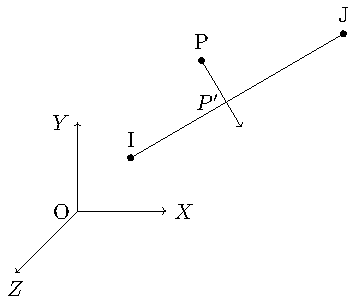
\includegraphics[height=0.3\textheight]{algo.pdf}
  %   \caption{CFD风压点$P$与梁单元$IJ$示意图}
  %   \label{fig:algo}
  % \end{figure}

  \begin{itemize}
  \item 
    判断风压点$P$是否作用于梁单元$IJ$上:
    \begin{columns}
      \column{0.7\textwidth}
      \begin{itemize}
      \item $P'$是否在线$IJ$内部?
        $$ \bm{P'I}\cdot\bm{P'J} < 0 $$
      \item $PP'$是否近似等于单元$IJ$外径?
        $$ |PP'-R_{IJ}| < \varepsilon $$
      \end{itemize}

      \column{0.3\textwidth}
      \begin{figure}[!htbp]
        \centering
        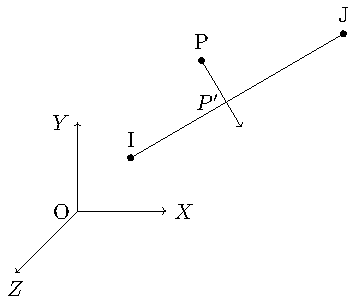
\includegraphics[width=0.8\textwidth]{algo.pdf}
        \caption*{CFD风压点$P$与梁单元$IJ$示意图}
        \label{fig:algo}
      \end{figure}

    \end{columns}

    \bigskip
  \item
   单个有限元梁单元所受所有CFD风压点的压力进行合成,并分配到该单元节点: 
   \begin{itemize}
   \item 计算单个有限元梁单元$IJ$受到的所有风压点处风压分量的平均$\bar{p_X},\bar{p_Y},\bar{p_Z}$;
	\item 将风压根据梁表面面积转化为合力$F_X=2\pi R_{IJ} |IJ| \bar{p_X}$,$Y,Z$方向类似;
	\item 将风压合力分量平分到梁单元$I$、$J$节点上。
  \end{itemize}
  \end{itemize}
  
\end{frame}

\begin{frame}
  \frametitle{输电塔支撑构件的龙卷风荷载计算}
  \begin{itemize}
    \item 支撑构件梁单元某节点受到的风荷载可由下式计算
      \begin{equation}
        \bm{F_w} = \frac{1}{2} \rho_a C_d A |U| \bm{U}
      \end{equation}
      式中,$\rho_a$为空气密度,$C_d$为体型系数,本文取为$1.0$,$A$为该节点迎风投影面积,$\bm{U}$为风场在该节点处的风速矢量。
      
      \bigskip
    \item 提取fluent 风场中任意节点风速的UDF程序算法:
      \begin{itemize}
      \item
	      首先判断出点$P$所在的计算流域网格控制体(可通过点$P$与某控制体各表面形心连线的向量与控制体表面法向量的关系判断点 是否属于该控制体);
      \item
	      提取该控制体的中心$C$点坐标$(x_c, y_c, z_c)$和$C$处的流场速度分量和速度梯度分量(将速度和各方向速度分量梯度矢量记为$\bm{U_C}$和$\bm{G_{CX}}$、$\bm{G_{CY}}$、$\bm{G_{CZ}}$);
      \item
	      利用下式计算点$P$处$X$方向速度分量为($Y$和$Z$方向速度分量可类似计算)
	      \begin{equation}
	      	U_{PX} = U_{CX} + (\bm{OP}-\bm{OC})\cdot \bm{G_{CX}}
	      \end{equation}
      \end{itemize}
    \end{itemize}
\end{frame}


\subsection{输电塔龙卷风荷载计算的规范方法}

\begin{frame}
  \frametitle{龙卷风风场处理}

  \begin{figure}[!htpb]
    \centering
    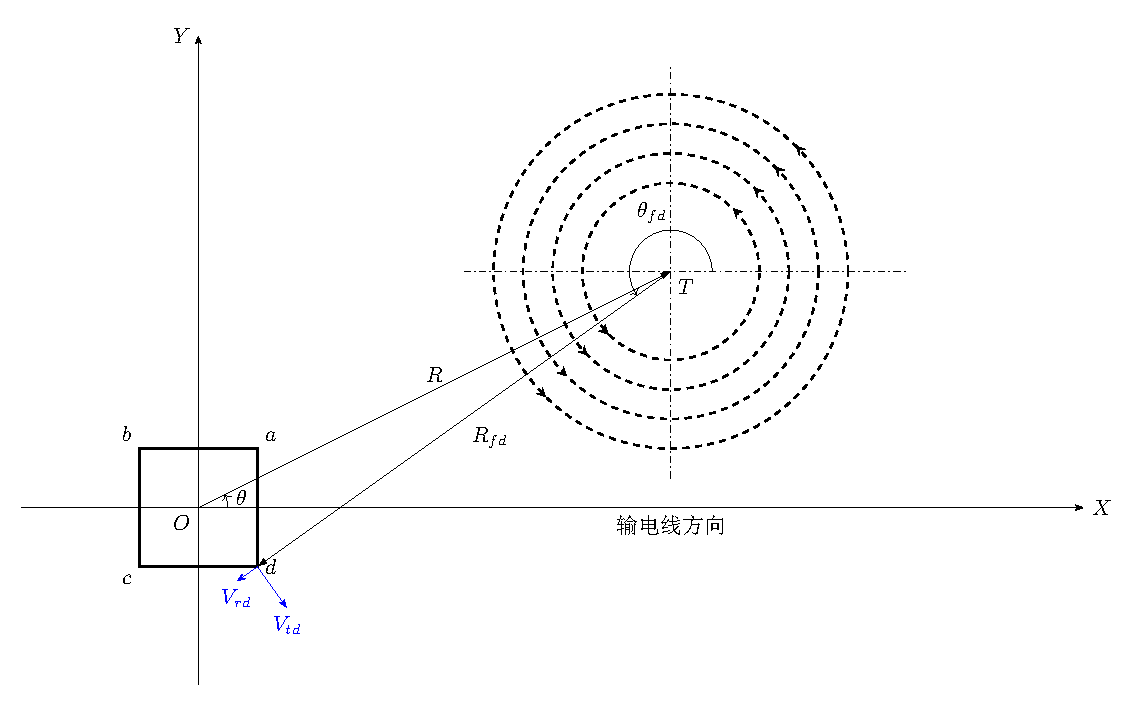
\includegraphics[width=\textwidth]{tower_tornado_cs.pdf}
    \caption*{输电塔在龙卷风风场中的水平投影示意图}
    \label{fig:tower-tornado-cs}
  \end{figure}

\end{frame}

\begin{frame}
  \frametitle{中国架空输电线路设计规范风荷载计算方法}
  \begin{equation}
    W_{\mathrm{s}} = W_{0} \cdot \mu_{\mathrm{z}} \cdot \mu_{\mathrm{s}} \cdot B_{2} \cdot A_{\mathrm{s}} \cdot \beta_{\mathrm{z}}
  \end{equation}
  \begin{equation}
    W_0 = V^2/1600
  \end{equation}
  \begin{description}
	\item[$W_{\mathrm{s}}$] 杆塔风荷载标准值(\SI{}{kN});
	\item[$W_{0}$] 基准风压标准值(\SI{}{kN/m^2});
	\item[$V$] 基准高度为\SI{10}{m}的风速(\SI{}{m/s});
	\item[$\mu_{\mathrm{z}}$] 风压高度变化系数
	\item[$\mu_{\mathrm{s}}$] 构件的体型系数,杆塔取$1.3(1+\eta)$,环形截面钢筋混凝土杆取$0.7$;
	\item[$B_{2}$] 杆塔构件覆冰风荷载增大系数,\SI{5}{mm}冰区取$1.1$,\SI{10}{mm}冰区取$1.2$,\SI{15}{mm}冰区取$1.6$,\SI{20}{mm}冰区取$1.8$,\SI{20}{mm}以上冰区取$2.0$~$2.5$;
	\item[$A_\mathrm{s}$] 迎风面构件的投影面积计算值(\SI{}{m^2});
	\item[$\eta$] 塔架背风面荷载降低系数;
	\item[$\beta_\mathrm{z}$] 杆塔风荷载调整系数。
  \end{description}
\end{frame}

\begin{frame}
  \frametitle{输电塔龙卷风荷载施加方法}
  \begin{figure}[!htbp]
    \centering
    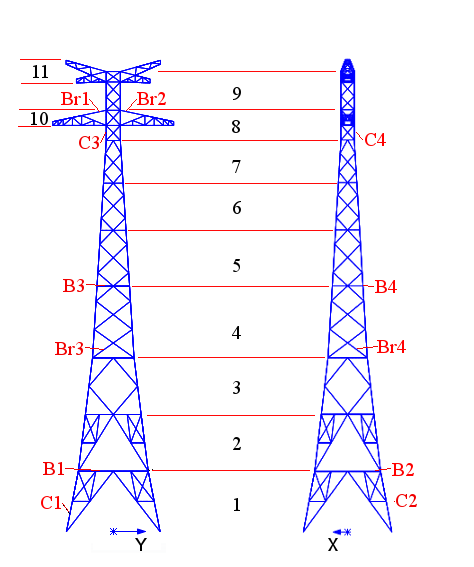
\includegraphics[height=0.8\textheight]{tower_zone.png}
    \caption*{输电塔分层示意图}\label{fig:tower-zone}
  \end{figure}
 
\end{frame}

\begin{frame}
  \frametitle{输电塔龙卷风荷载施加方法}
  \begin{itemize}
  \item 计算输电塔节点a,b,c和d处龙卷风速度分量 $V_x$和$V_y$;
  \item 分别沿$X$和$Y$方向计算风速风量的均值$V_x'$和$V_y'$;
  \item 计算输电塔节点a,b,c和d处所在层龙卷风荷载
    \begin{equation}
      F_{\mathrm{w}x} = 0.625 (V_{x}')^2 \mu_{\mathrm{s}x} A_x 
    \end{equation}
    \begin{equation}
      F_{\mathrm{w}y} = 0.625 (V_{y}')^2 \mu_{\mathrm{s}y} A_y 
    \end{equation}
  \item 迎风面和背风面上风荷载分配
     中国规范根据塔架背风面荷载降低系数$\eta$对某层输电塔所受风荷载进行分配,即迎风面节点在$X$和$Y$方向所受风荷载分量分别为 $1/(1+\eta) F_{\mathrm{w}x}$ 和 $1/(1+\eta) F_{\mathrm{w}y}$;背风面节点在$X$和$Y$方向所受风荷载分量分别为 $\eta/(1+\eta) F_{\mathrm{w}x}$ 和 $\eta/(1+\eta) F_{\mathrm{w}y}$;
   \item 迎(背)风面节点间风荷载分配
     迎(背)风面上的节点根据各节点的投影面积进行迎(背)风面上风荷载的分配。
   \end{itemize}
\end{frame}

\subsection{FSI方法与规范方法的对比}

\begin{frame}
  \frametitle{FSI方法与规范方法的对比}
  
  \begin{columns}
    \column{0.5\textwidth}
    \begin{figure}[!htbp]
      \centering
      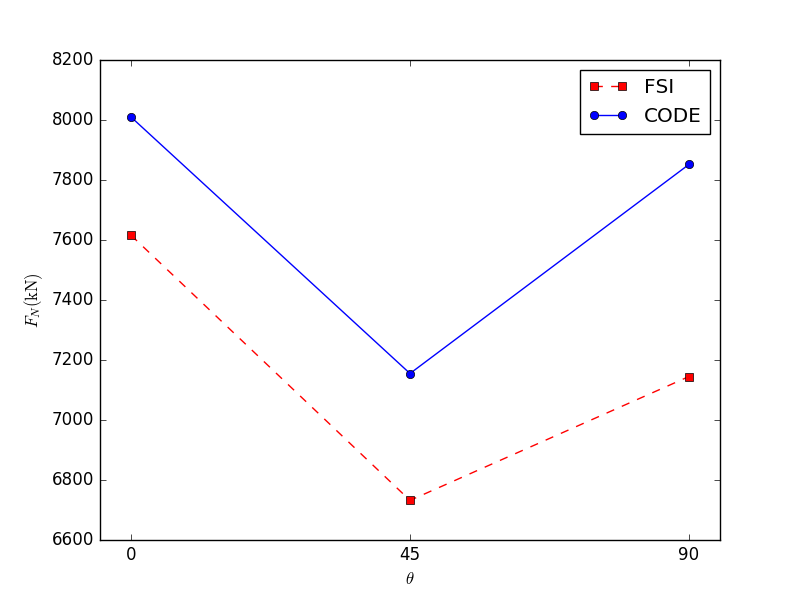
\includegraphics[width=\textwidth]{Fx_vs_theta.png}
      \caption*{输电塔构件最大轴向压力随袭击角的变化}
      \label{fig:fx-vs-theta}
    \end{figure}

    \column{0.5\textwidth}
    \begin{figure}[!htbp]
      \centering
      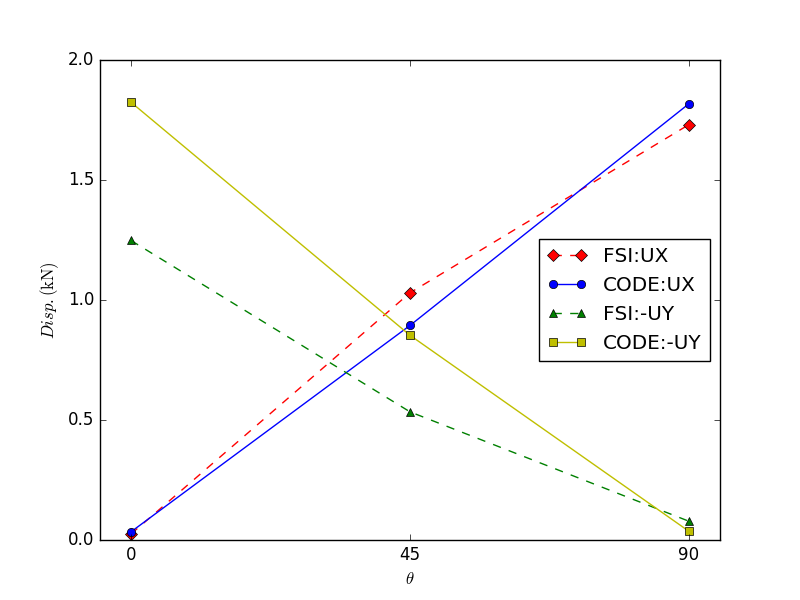
\includegraphics[width=\textwidth]{Disp_vs_theta.png}
      \caption*{输电塔构件最大位移分量随袭击角的变化}
      \label{fig:disp-vs-theta}
    \end{figure}

  \end{columns}
\end{frame}

\begin{frame}
  \frametitle{FSI方法与规范方法的对比}
  \begin{table}[!htbp]
    \caption*{输电塔代表构件的轴向力}
    \label{tab:axial-force}
    \centering
    \begin{tabu} to 1.0\textwidth {X[c] X[c] X[3,c] X[2,c] X[3,c] X[2,c]}
      \toprule
      \multicolumn{2}{c}{构件} & \multicolumn{2}{c}{单向流固耦合} & \multicolumn{2}{c}{规范方法} \\
      编号 & 类型 & $F_N$(\SI{}{kN}) & 角度(\SI{}{\degree}) & $F_N$(\SI{}{kN}) & 角度(\SI{}{\degree}) \\
      \midrule
      C1	& 柱	& -6485	& 90 & 	-7803	& 90  \\
      C2	& 柱	& 7739	& 0	 &   8154	& 0  \\
      C3	& 柱	& -4958	& 90 &	-5024	& 90  \\
      C4	& 柱	& 5700	& 0	 &   5762	& 0  \\
      B1	& 梁	& 328	& 90 &	488	    & 90  \\
      B2	& 梁	& -274	& 0	 &  -316	& 0  \\
      B3	& 梁	& 87	& 0	 &   120	& 90  \\
      B4	& 梁	& -123	& 90 &	-130	& 90  \\
      Br1	& 支撑	& -27	& 45 &	-51	    & 45  \\
      Br2	& 支撑	& -42	& 45 &	-71	    & 45  \\
      Br3	& 支撑	& 318	& 90 &	588	    & 90  \\
      Br4	& 支撑	& -268	& 0	 &  -371	& 0  \\
      \bottomrule
    \end{tabu}
  \end{table}

\end{frame}

\section{考虑龙卷风平移效应的动态响应分析}
\subsection{动态龙卷风模型}

\begin{frame}
  \frametitle{动态龙卷风模型}
  \begin{itemize}
  \item 
    假定龙卷风核心在地面上做匀速直线运动,描述其路径的关键参数为核心初始位置和运动速度
    \begin{itemize}
    \item
      若初始时刻龙卷风核心距离输电塔很近,结构会受到量值很大的突加荷载的影响,与实际情况不符,需要将龙卷风核心初始位置设置在距离输电塔较远的地方。
      初始位置在整体坐标系中的位置记为$\left(x^T_{0},y^T_{0}\right)$。
    \item
      假设龙卷风平移速度为$v^T=\SI{20.0}{m/s}$;
      平移速度相对于输电线、即$X$轴正向的夹角为$\theta^T$。
   
    \end{itemize}
  
  \end{itemize}

  \begin{figure}[!htpb]
    \centering
    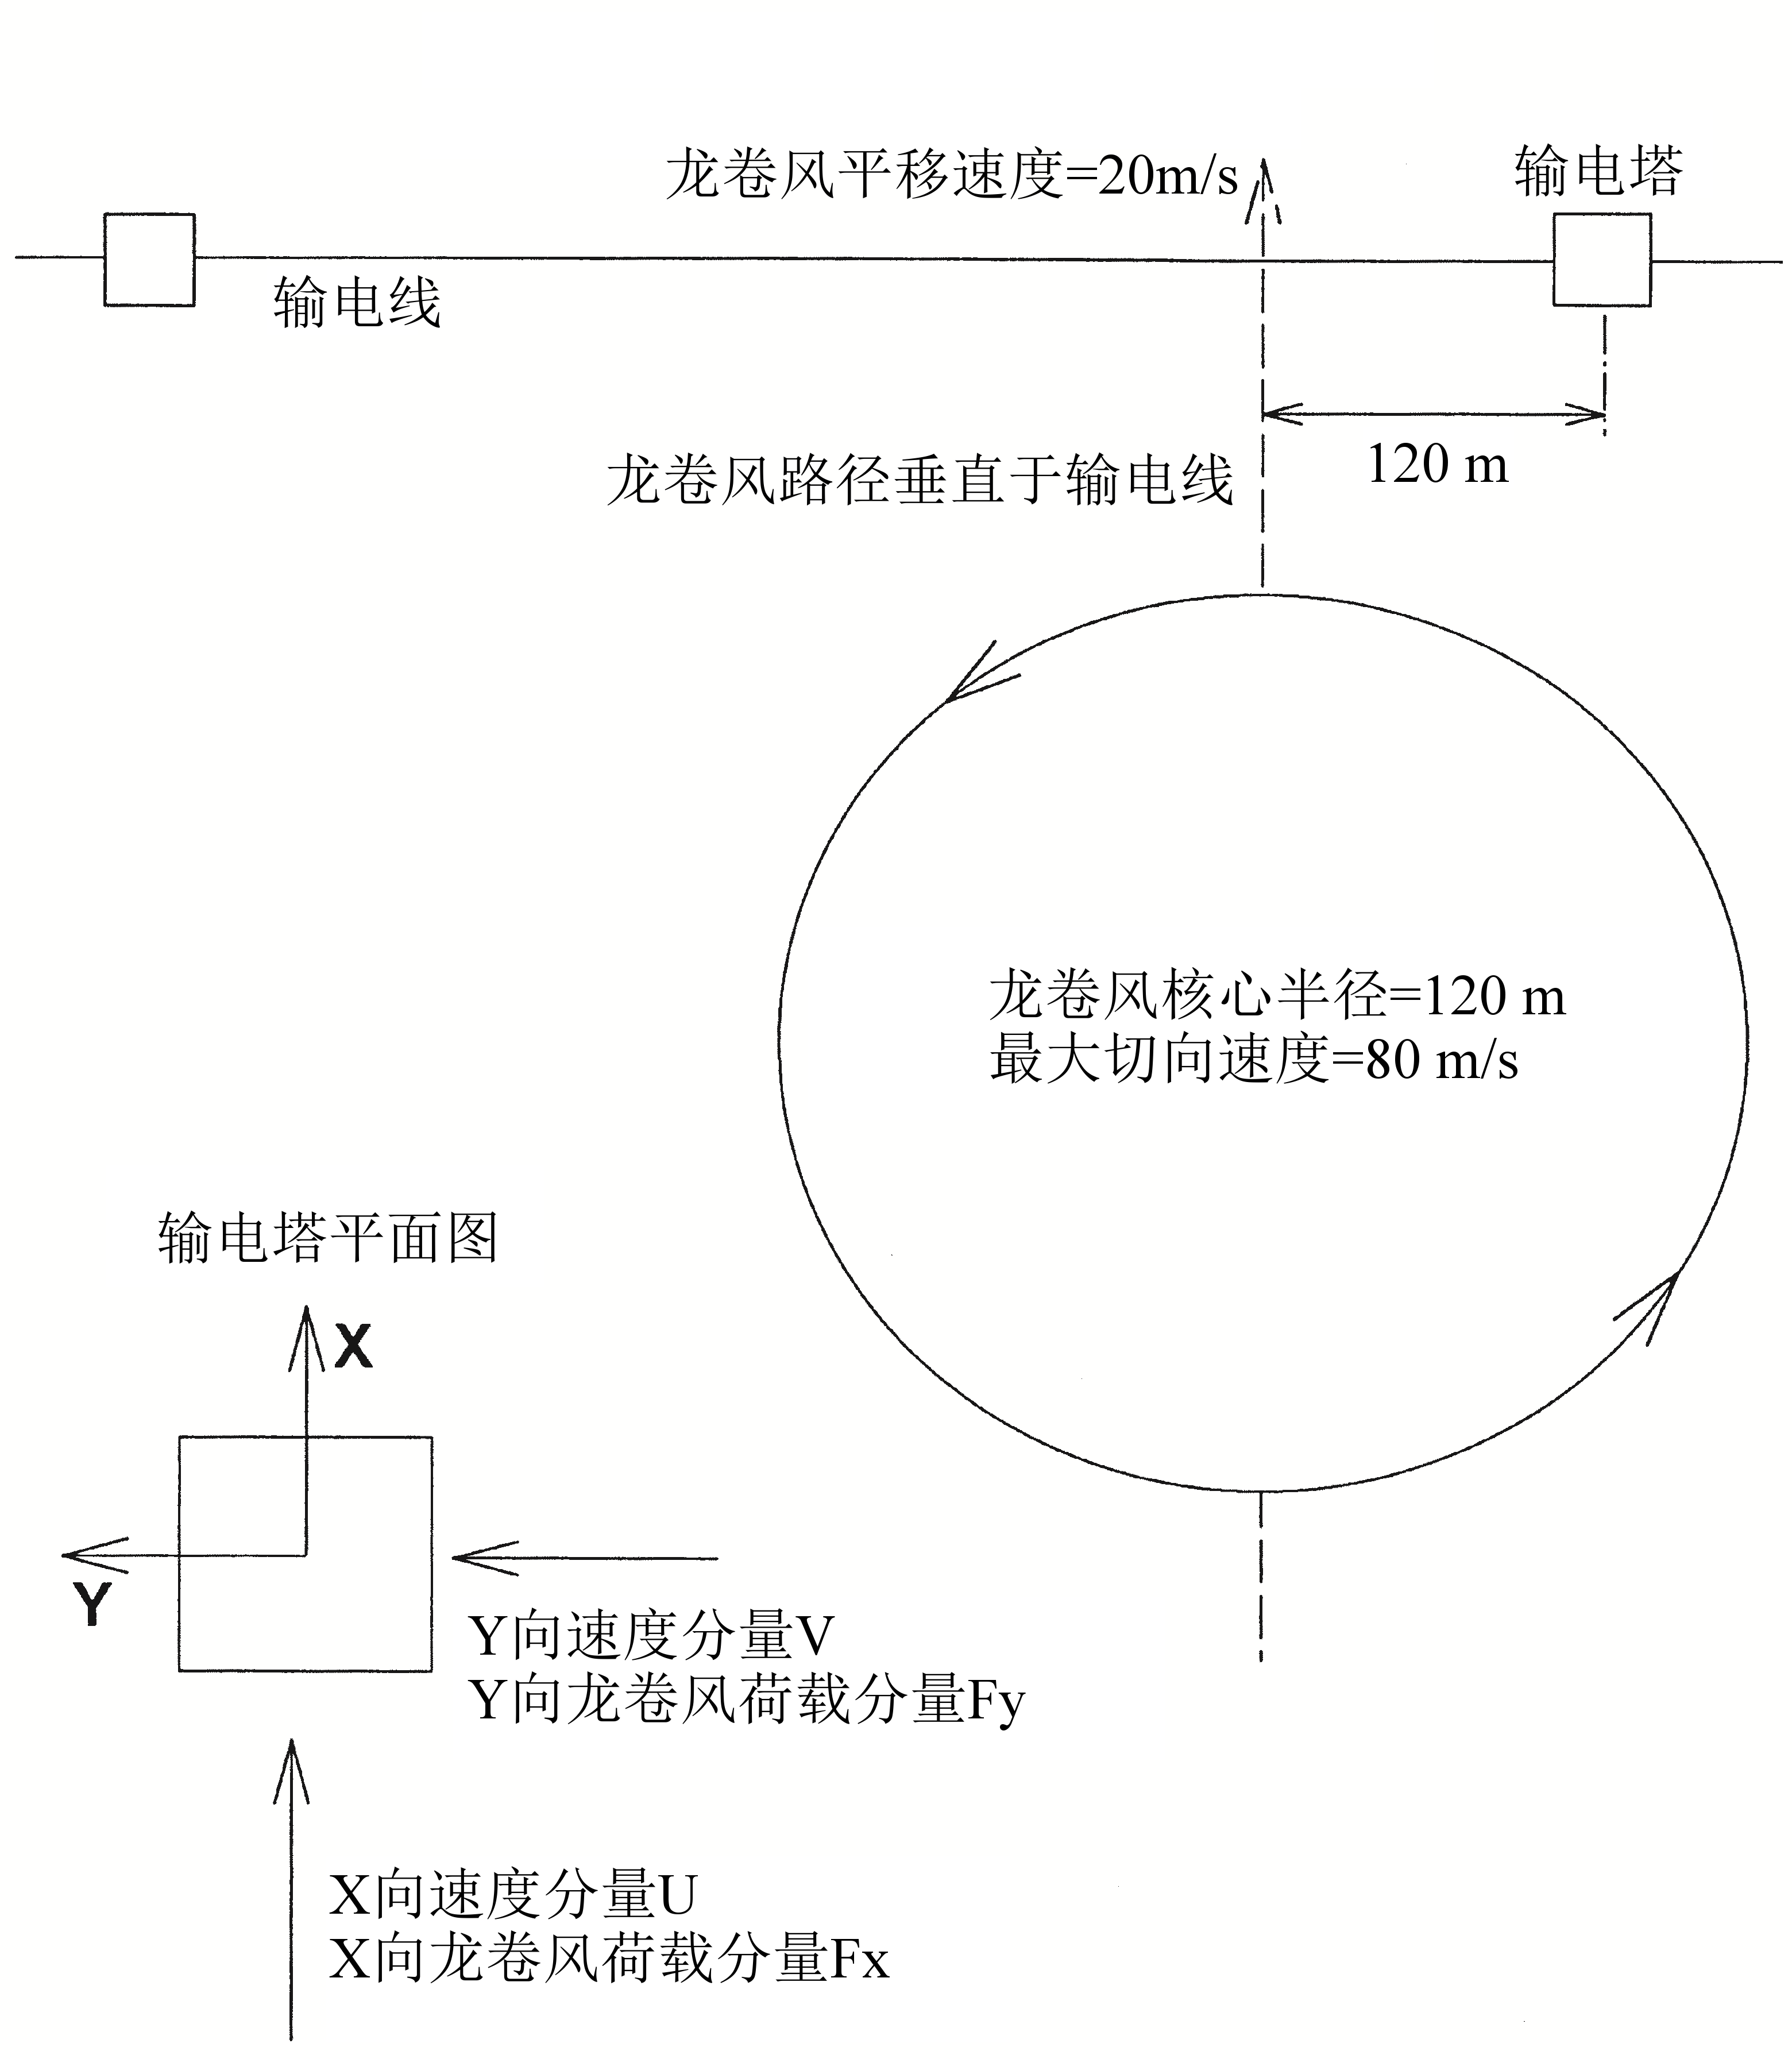
\includegraphics[height=0.5\textheight]{tornado-path.png}
    % \caption{龙卷风相应于输电塔做平移运动的示意图}
    \label{fig:tornado-path}
  \end{figure}
\end{frame}

\subsection{动态龙卷风风速和荷载时程}

\begin{frame}
  \frametitle{龙卷风平移工况}
  \begin{figure}[!htpb]
    \centering
    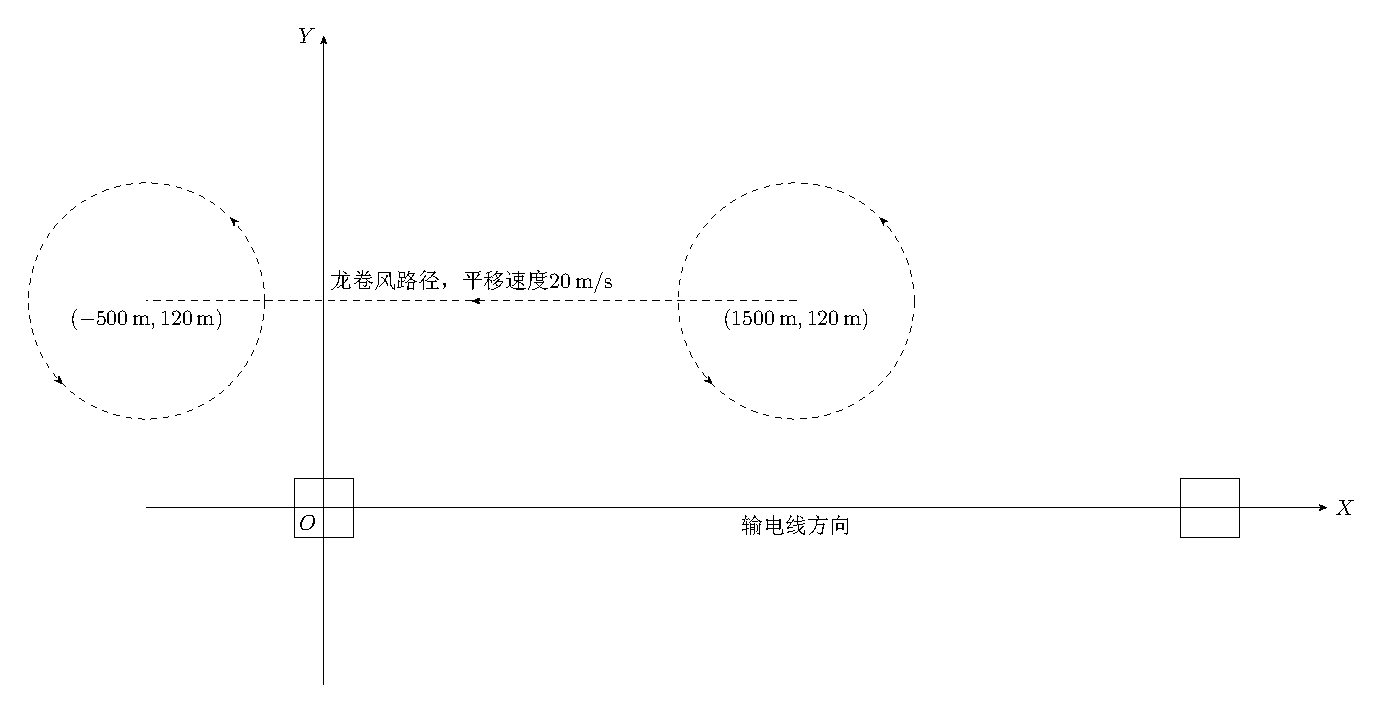
\includegraphics[height=0.7\textheight]{dynamic-case1.pdf}
    \caption*{龙卷风平行运动工况}
    \label{fig:dynamic-case1}
  \end{figure}
\end{frame}

\begin{frame}
  \frametitle{龙卷风平移工况风速和荷载时程}
  \begin{columns}
   \column{0.5\textwidth}
   \begin{figure}[!htpb]
     \centering
     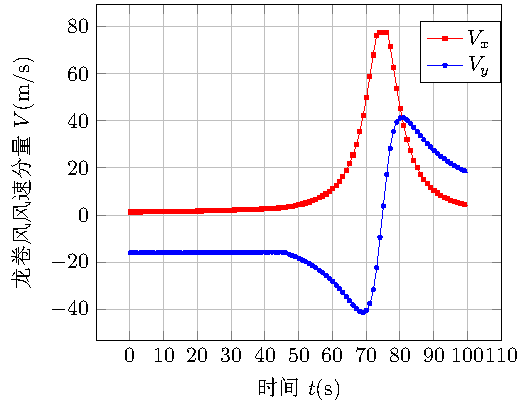
\includegraphics[width=0.8\textwidth]{velo_case1.pdf}
     \caption*{龙卷风运动平行工况塔顶节点风速时程}
     \label{fig:velo_case1}
   \end{figure}
   \column{0.5\textwidth}
   \begin{figure}[!htpb]
     \centering
     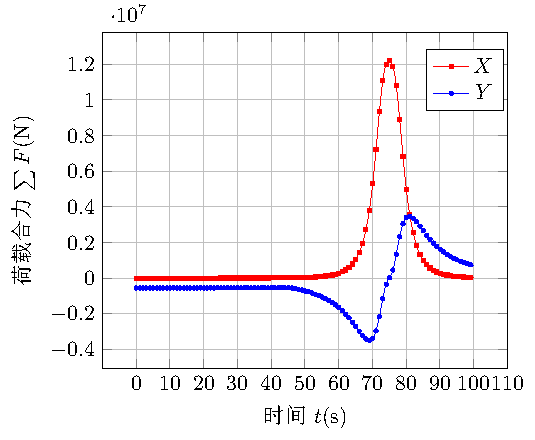
\includegraphics[width=0.8\textwidth]{sum_f_case1.pdf}
     \caption*{龙卷风运动平行工况荷载分量合力时程}
     \label{fig:sum_f_case1}
   \end{figure}
  \end{columns}
\end{frame}

\begin{frame}
  \frametitle{龙卷风垂直工况}
  \begin{figure}[!htpb]
    \centering
    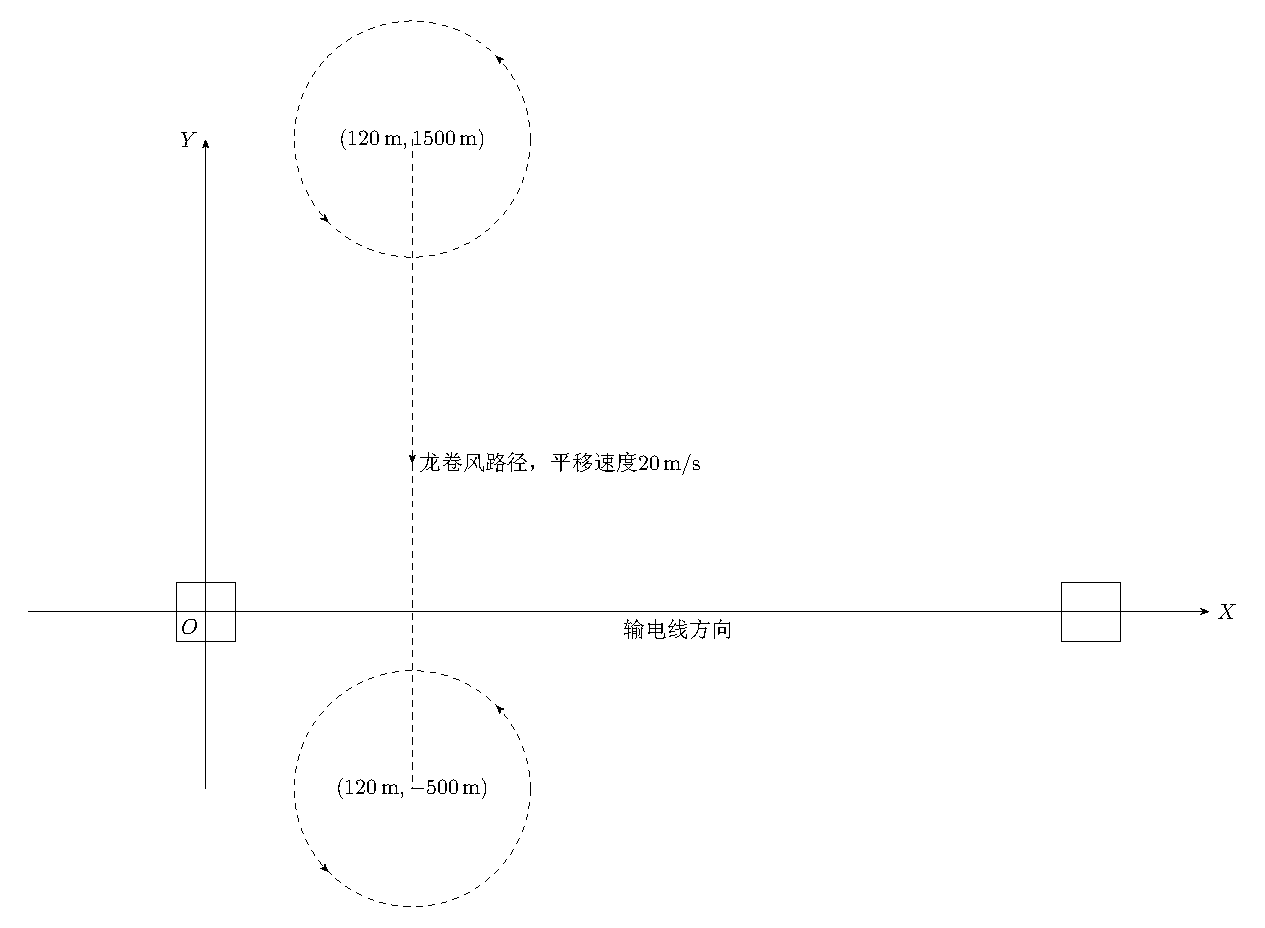
\includegraphics[height=0.7\textheight]{dynamic-case2.pdf}
    \caption*{龙卷风垂直运动工况}
    \label{fig:dynamic-case2}
  \end{figure}
\end{frame}

\begin{frame}
  \frametitle{龙卷风垂直工况风速和荷载时程}
  \begin{columns}
   \column{0.5\textwidth}
   \begin{figure}[!htpb]
     \centering
     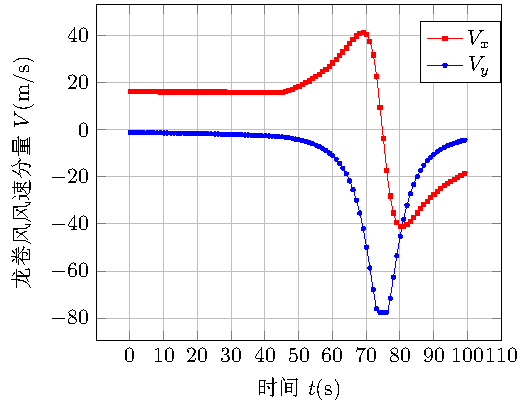
\includegraphics[width=0.8\textwidth]{velo_case2.pdf}
     \caption*{龙卷风运动垂直工况塔顶节点风速时程}
     \label{fig:velo_case2}
   \end{figure}
   \column{0.5\textwidth}
   \begin{figure}[!htpb]
     \centering
     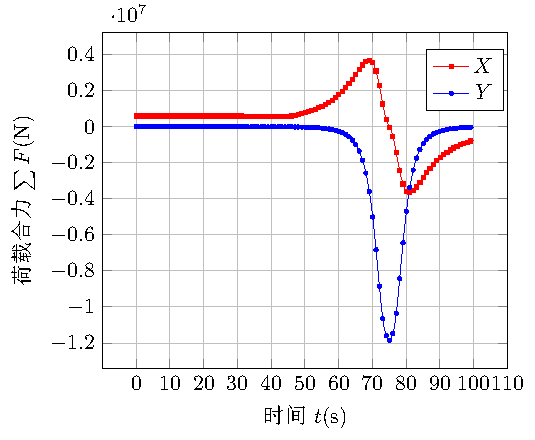
\includegraphics[width=0.8\textwidth]{sum_f_case2.pdf}
     \caption*{龙卷风运动垂直工况荷载分量合力时程}
     \label{fig:sum_f_case2}
   \end{figure}
  \end{columns}
\end{frame}

\subsection{输电塔结构动力时程分析}

\begin{frame}
  \frametitle{输电塔动态响应结构}
  \begin{columns}
   \column{0.5\textwidth}
   \begin{figure}[!htpb]
     \centering
     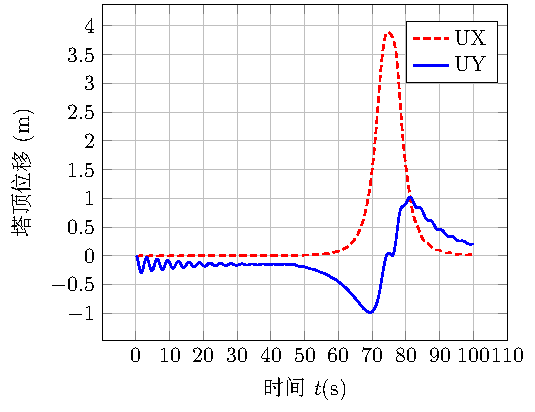
\includegraphics[width=0.8\textwidth]{disp_top_case1.pdf}
     \caption*{龙卷风运动平行工况塔顶节点位移响应时程}
     \label{fig:disp_top_case1}
   \end{figure}
   \column{0.5\textwidth}
   \begin{figure}[!htpb]
     \centering
     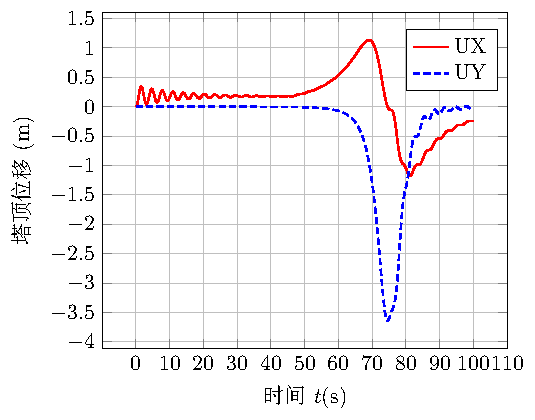
\includegraphics[width=0.8\textwidth]{disp_top_case2.pdf}
     \caption*{龙卷风运动垂直工况塔顶节点位移响应时程}
     \label{fig:disp_top_case2}
   \end{figure}
  \end{columns}
\end{frame}

\section{课题总结与展望}

\begin{frame}
  \frametitle{课题研究结论}
  \begin{itemize}
  \item
    依据文献中龙卷风试验模拟为基础建立了 CFD 缩尺龙卷风风场,发现缩尺风场的切向风速的分布与 Rankine涡模型及试验测得的风速分布吻合较好。
  \item
    通过长度相似比和速度相似比的概念可将缩尺风场模型改造成足尺龙卷风风场模型。
  \item
    采用单向流固耦合和规范方法计算得到的输电塔结构轴向力和位移响应随龙卷风袭击角的变化趋势相似,且FSI方法计算的结构最大轴向力响应小于规范方法,且误差不大于$20\%$。
  \item
    考虑龙卷风平移效应的动态响应分析,平行工况下龙卷风荷载总和时程在输电线方向的分量出现持续时间约为\SI{10}{s}的波形(荷载先逐渐增大,后逐渐衰减),且荷载峰值较大,呈现出一定的冲击效应。
  \end{itemize}
\end{frame}

\begin{frame}
  \frametitle{课题研究展望}
  \begin{itemize}
  \item
    实测的龙卷风存在多涡形态,且受地面粗糙度,研究者认为实测的龙卷风涡流比约为$2.0$,本文模拟的风场涡流比为$0.28$,故本文模拟的数值龙卷风与实际情况存在差距。今后可考虑通过引入更为精细的数值模拟方法(如大涡模拟等),以模拟出更为符合实际的龙卷风风场。

  \item
    本文忽略了输电线受到的龙卷风作用,这主要是考虑到龙卷风尺度相比输电线长度较小,且输电线受到的风荷载作用机理较为复杂。
    本文还忽略了输电线与塔的耦合作用,这种耦合作用在动力时程分析中会产生较大的阻尼,但考虑这一作用会引起结构有限元分析的较强非线性。
    今后的研究可考虑输电线受到的龙卷风荷载和输电线与塔的耦合作用。

  \item
    本文中龙卷风作用下输电塔结构的准静态分析考虑了结构材料非线性和几何非线性,但考虑龙卷风移动效应的动力时程分析中假定结构处于弹性状态。
    今后的研究可考虑动力时程分析中结构的材料非线性和几何非线性,进而进行倒塌性分析。

  \item
    真实的龙卷风风场中风致飞射物对结构的打击作用不容忽视,也是造成结构破坏的一个重要因素。
    本文未考虑风致飞射物的影响。
  \end{itemize}
\end{frame}

\thankyoupage{感谢各位老师和同学出席!}

% \end{CJK*}
\end{document}
